\documentclass[conference]{IEEEtran}

\usepackage{cite}
\usepackage{amsmath,amssymb,amsfonts}
\usepackage{graphicx}
\usepackage{textcomp}
\usepackage{multirow}
\usepackage{hyperref}
\usepackage{booktabs}
\usepackage{algorithm}
\usepackage{algpseudocode}
\usepackage{subcaption}
\usepackage{lipsum} % For lipsum
\usepackage[dvipsnames]{xcolor} % Custom Colors
\definecolor{mygray}{gray}{0.6} % Definining a .6 transparency gray called mygray
\setlipsum{% Making the lipsum text mygray
  par-before = \begingroup\color{mygray},
  par-after = \endgroup
}
\newcommand{\probP}{\text{I\kern-0.15em P}}
\newcommand{\tl}[1]{\textit{[{\color{red}#1}]}}
\newcommand{\cm}[1]{\textit{{\color{blue}#1}}}
\newcommand{\erik}[1]{\textit{[{\color{brown}Erik: #1}]}}
\newcommand{\mr}[1]{\textit{[{\color{brown}Mohammed: #1}]}}

\begin{document}

%%
%% The "title" command has an optional parameter,
%% allowing the author to define a "short title" to be used in page headers.
\title{A Tiny, Human-Interpretable, Client-Side, Classifier}

%%
%% The "author" command and its associated commands are used to define
%% the authors and their affiliations.
%% Of note is the shared affiliation of the first two authors, and the
%% "authornote" and "authornotemark" commands
%% used to denote shared contribution to the research.

\author{
    \IEEEauthorblockN{Charles Meyers}
    \IEEEauthorblockA{Umeå University\\
    % Umeå, Sweden\\
    \email{cmeyers@cs.umu.se}}
    
    \IEEEauthorblockN{Aaron P. MacSween}
 
    
    \IEEEauthorblockN{Tommy Löfstedt}
    % \IEEEauthorblockA{Umeå University\\
    % Umeå, Sweden\\
    % \email{tommy@cs.umu.se}}
    
    \IEEEauthorblockN{Erik Elmroth}
%     \IEEEauthorblockA{Umeå University\\
%     Umeå, Sweden\\
%     \email{elmroth@cs.umu.se}}
}

\maketitle

\begin{abstract}
% Machine learning has proven remarkable performance across a wide variety of domains, but can nevertheless fail to adversaries during model training or deployment.
\cm{
In recent years, developments in machine learning have highlighted a conflict between platforms and their users in terms of privacy. 
The importance of user privacy and the struggle for power over their data has been intensified as regulators and platform operators attempt to police their platforms while respecting the privacy of users. 
Client-side data storage, management, and analysis has become the favoured approach to large scale machine learning. 
Whether client-side or in the cloud, these state of the art methods require vast amounts of labelled user data, making them unsuitable for models that only have access to a single user's data. 
Also, state of the art methods are computationally expensive, which degrades user experience on compute limited hardware and reduces battery life. 
Older machine learning methods often require fewer samples to be effective, but generally have a reduced ability to model complex decision boundaries. 
An alternative approach that uses compression algorithms to measure the distance between two objects in conjunction with classical machine learning methods has proven remarkably successful at classification tasks across a wide-variety of datasets—using only a small number of samples. 
In this work, we present techniques for improving the run-time characteristics of this compression-based metric and frame this distance measure in the wider context of kernel metrics to allow the modelling of complex decision boundaries using only a small number of samples. 
We show that this compression metric outperforms all tested string metrics--without incurring additional computational cost. 
The end results is a simple, client-side, spam detection model that competes with state of the art models while requiring only a fraction of the power and data and compute requirements, and nevertheless competes with the state of the art models.
}
\end{abstract}





\section{Introduction}

Despite their efficacy across many domains, modern machine learning methods often use very large models that require large numbers of samples to train~\cite{desislavov2021compute}.  
\cm{Generally this data is collected from the end-user using dubious amounts of consent~\cite{nouwens2020dark} and aggregated at massive scales~\cite{desislavov2021compute} to train these massive models.} 
The collection of this data often creates privacy and security risks~\cite{chakraborty_adversarial_2018,meyers}. 
For example, several attacks against ML systems have been proposed, targeting the model during training~\cite{biggio_poisoning_2013}, prediction~\cite{biggio_evasion_2013,deepfool,carlini_towards_2017}, or deployment~\cite{distributed_attacks,santos2021universal}.
Even when access to a model is limited only to the classification labels, it is possible to subvert the model~\cite{hopskipjump}, reverse engineer the decision boundary~\cite{deepfool}, determine the model weights~\cite{jagielski2020high} or infer the class-membership of new samples~\cite{bentley2020quantifying}. 
This raises profound questions for safety critical systems~\cite{meyers} and legal questions about access and control of the underlying data~\cite{mitrou2018data,marks2023ai}. 
\cm{
Furthermore, regulators and platform operators around the world have sought to balance privacy and security concerns by weakening encryption standards ~\cite{amnesty_encryption} or by scanning client devices for offensive content using neural networks~\cite{chat_control} that are known to leak private data~\cite{xiao2021improving,fredrikson_model_2015} while being trivial to circumvent with adversarial queries ~\cite{carlini_towards_2017,dohmatob_generalized_2019,hopskipjump,biggio_evasion_2013,meyers,chakraborty_adversarial_2018}.
}
One solution to the problem of adversaries is to treat the model as we would treat a session token or any other private data---by keeping it encrypted locally and providing no access in either direction to the internet (\textit{i.e.} keep private data \textit{private}).
However, this lack of data sharing means that this hypothetical method must work well when trained on a data collected from a single user.

Recently, Jiang \textit{et al.}~\cite{jiang2022less} proposed a parameter-free text classification algorithm (NCD-KNN) that exploits the distance measure, \textit{normalized compression distance} (NCD)~\cite{ncd},  to classify objects using the k-nearest neighbours (KNN) algorithm~\cite{shalev2014understanding}.
This method has shown very strong performance across several benchmark datasets, but the choice of KNN over other simple models is seemingly unexplored and unjustified. 
\cm{
Instead of relying on massive amounts of centralised data, this work proposes a model that has remarkable efficacy on a small number of samples and can be trained and queried entirely on a client device in real time.
In this study, we explore the underlying theory of kernel methods and extend this notion of distance (dissimilarity) to one of kernel-like similarity}; offer run-time improvements over Jiang's method~\cite{jiang2022less}; and demonstrate the efficacy of our run-time optimised method on a variety of datasets to produce a model that competes with state-of-the-art neural network models trained on much larger datasets.  ~\cm{
The end result is a method that can run entirely on a client device without federation or centralisation of data across many users, allowing platform operators to find malicious users without exfiltrating private data from the entire user base.
}




\subsection{Threat Model}
\label{threat}

A typical machine learning pipeline is vulnerable to attacks that target each stage of the machine learning pipeline. Broadly speaking, they come in white- and black-box categories~\cite{meyers}. White-box attacks like the fast gradient method~\cite{fgm} or Deepfool~\cite{deepfool} require access to the model directly while other attacks can succeed with only normal API access. 
Additionally, it has been shown that finding prototypical meta samples from the training set of neural networks is trivial~\cite{chakraborty_adversarial_2018}. 
Likewise, this class membership data can then be used to reverse engineer the model weights~\cite{deepfool} and loss gradients for a set of (potentially adversarial) examples~\cite{hopskipjump}. 
Even if the attacker only has access to a typical application programming interface (API), there are effective adversarial attacks\cite{hopskipjump}. 
In short, the federated and centralized training paradigms are inherently fragile to attackers and dangerous for user privacy, even if the resulting model lives on the user device (rather than in the cloud). 
Instead of relying on a model trained on massive amounts of user data, as is typical in deep neural networks and other ``big data'' approaches, we can categorically sidestep these attacks with a model that runs entirely client-side. 
By avoiding the typical model-as-a-shared-service approach, the attack surface is reduced to only adversaries that have access to data that users generally consider private (\textit{e.g.}, the contents of a message). 
That is, the attack surface is reduced to that of any other cookie or browser-based secret~\cite{} and can be unique to each user, session, or device by collecting data from each user and training a model on a client device.



\subsection{Motivations} 

There are several motivations for this work. 
First, \textit{normalized compression distance} (NCD) has been demonstrated to be a \textit{universal} measure of similarity between two objects~\cite{ncd}.
Secondly, Jiang's analysis~\cite{jiang2022less} relies on many thousands of samples and it's unclear how well it performs in few-shot circumstances or in the case of extremely imbalanced data (\textit{e.g.} malicious user datasets).
While follow-up research examined topics like image classification~\cite{opitz2023gzip}, chemical classification~\cite{weinreich2023parameter}, and text classification~\cite{nishida2011tweet}, its ability to separate malicious users from benign ones remains unexplored. 
Thirdly, we can expand this notion of distance (\textit{e.g.} dissimilarity) to a kernel space that measures similarity in an attempt to use this technique with more complicated algorithms than the KNN proposed by Jiang~\cite{jiang2022less} to allow for non-linear decision boundaries. 
Furthermore, if run-time storage and computation requirements are minimal, then we can fulfill our goal of deploying this method entirely client-side.
In the simplest case, that might mean marking an email as spam~\cite{ansuz_email} or examining the nearest neighbours in a browser~\cite{ansuz_browser}. The goal of the work is to produce a human-interpretable model with comparable accuracy that can be trained on and used by each user in isolation from all others, categorically circumventing the privacy and security concerns associated with the collection of millions of user-generated data points.



\subsection{Contributions}
In this study, we:

\begin{itemize}
    \item Explore the theory behind normalized compression distance as a pseudo-metric.
    \item Demonstrate how private model deployment is safer by design (Sec.~\ref{threat}) and their efficacy on several datasets.
    \item Offer run-time improvements over the NCD-KNN classifier (Sec.~\ref{improvements}).
    \item Provide a \texttt{javascript} as well as a \texttt{scikit-learn}-compatible \texttt{python} implementation of these compression-based classification models.
    \item Demonstrate the efficacy of the NCD-based classifiers across several binary classification datasets.
\end{itemize}





\section{Background}

In the sections below, we outline the definition of a metric space and the connection to normalized compression distance (NCD), briefly explore the run-time of k-Nearest Neighbour (KNN) classifiers, and give a high-level overview of the tested compression algorithms.



\subsection{Measures of Distance}

\cm{There are many different ways to measure the dissimilarity (or distance) between two objects.}
For strings, several measures of distance are routine and available via the \texttt{levenshtein} package~\cite{levenshtein}. 
The set of evaluated string metrics is outlined in Sec.~\ref{string_metrics}. 
A somewhat forgotten method, proposed in 2001~\cite{ncd} (see Section~\ref{ncd}) extends to any type of object (not just strings) and a modified version of this metric has been incorporated into malware analysis tools for nearly two decades~\cite{}. 
Jiang \textit{et al.} ~\cite{jiang2022less} propose using this distance measure in conjunction with the KNN classifier, but this method is identical to other classifiers~\cite{vapnik1994measuring} that use measures of distance to cluster samples into classes. 



\subsubsection{Normalized Compression Distance}
\label{ncd}

The normalized compression distance~\cite{ncd} (NCD) is defined as:
\begin{equation}
    \text{NCD}(x, y) = \frac{\mathcal{C}(xy) - \min[\mathcal{C}(x), \mathcal{C}(y)]}{\max[\mathcal{C}(x), \mathcal{C}(y)]} + \varepsilon,
\end{equation}
where $\mathcal{C}(z)$ is the length (in bits) of the compressed form of the data $z$ using a compression algorithm, $xy$ denotes the concatenation of strings $x$ and $y$, and $\varepsilon$ is an error term due to imperfect compression algorithms~\cite{ncd}. This error is generally assumed to to be small relative to the rest of the terms and the original authors denote that the resultant NCD value can yield values larger than one~\cite{ncd}. To the best of our knowledge, nobody has addressed the problem of negative values for NCD\@. % The \@ signals to my linter that this is the end of a sentence and not an abbreviation. The linter can also handle stuff like \textit{e.g.} vs e.g. vs eg, hyper-parameter vs hyperparameter, etc. It's very useful and doesn't make automated changes (like a python linter would). 
Nevertheless, it has been used for classification tasks many times~\cite{opitz2023gzip,weinreich2023parameter,nishida2011tweet,jiang2022less} where the error term is simply assumed to be irrelevant since each of theses authors neglect to mention it.



\subsubsection{Other measures of string distance}
\label{string_metrics}

In addition to the NCD metric defined above, we examined several other measures of string similarity, widely used in natural language processing (NLP) and these are briefly outline below. 
% String Distances
\begin{itemize}
    \item \textit{Levenshtein:} the "edit distance" or minimum number of single-character edits to transform one string into another~\cite{navarro2001guided}.
    \item \textit{Ratio:} is one minus Levenshtein distance divided by the total length of the strings~\cite{levenshtein}.
    % \item \textit{SeqRatio:} identical to "Ratio", but calculated on sequences of strings by taking the single input string and splitting it into a list around white-space characters~\cite{levenshtein}.
    \item \textit{Hamming:} is the number of character positions where two strings differ, but is only defined for strings of equal length, leading to sparse distance matricies~\cite{hamming_distance}.
    % \item \textit{Jaro:} is a measure of similarity between two strings, taking into account the number of identical characters as well as the number of transposed characters~\cite{jaro}.
    % \item \textit{Jaro-Winkler:} extends the above by incorporating a scaling factor to give weight to sub-strings that occur more frequently~\cite{jaro}. 
\end{itemize}



\subsubsection{Metric Spaces}

A metric space is defined as some measure of distance between the constituent components of some space, usually called points.  For points $x_1,x_2...x_n \in X$ in a metric space, separated by distance $d(x_1,x_2)$, $d$ is a proper metric if and only if the following 4 identities are true~\cite{metrics}, each of which is given a label (which we've denoted in the parentheses):

\label{metric_spaces}
\begin{itemize}
    \item $d(x_1,x_2) = 0 \iff x = y$ (zero identity)
    \item $d(x_1,x_2) \geq 0$ (non-negativity identity)
    \item $d(x_1,x_2) = d(y, x)$ (symmetry identity)
    \item $d(x_1, x_3) \leq d(x_1,x_2) + d(x_2,x_3)$ (triangle inequality).
\end{itemize}
This metric space is often given the notation $M(X,d)$ since it is defined by the set, $X$, and the distance function, $d$.
In addition, we use the following notation to denote an inner product
$$
\langle \cdot , \cdot \rangle : V \times V \rightarrow \mathbb{R}
$$

for a vector space, $V$, and the field of real numbers, $\mathbb{R}$. 
Vector spaces, by definition are, at least, positive semi-definite such that for any (real-valued) vector, $X$, 
\begin{equation}
\langle X, X \rangle \geq 0
\label{eq:psd}
\end{equation}

\subsubsection{Mercer's Theorem and Kernelisation}
\label{kernels}
Whereas distance functions are used to measure the similarity between different examples $x,y$, a \textit{kernel-function}, $K$, is a measure of similarity. That is, when $d(x,x') = 0, x = y$ , but when $K(x,x') = 0, x~\perp~y$. The opposite then follows when $d(x,x')=1$ or $K(x,x')=1$. Mercer's theorem says that for any symmetric, continuous function, $K$,
$$
K : [a, b] \times [a, b] \rightarrow \mathbb{R}~\forall~x,x' \in [a,b].
$$
$K$ is said to \textit{positive semi-definite} if and if only for any set of points, $\{x_1, x_2, \cdots x_n\}$, and any set of real numbers, $\{ c_1, c_2 \cdots c_n\}$, then
\begin{equation}
\sum_{i=1}^n \sum_{j=1}^n K(x_i, x_j) c_i, c_j \geq 0.
\label{eq:mercers_theorem}
\end{equation}
That is to say, Equations~\ref{eq:psd}~\&~\ref{eq:mercers_theorem} are equivalent statements when 
$$
K(x, x') = \langle \phi(x), \phi(x') \rangle \nu
$$
where $\nu$ is the feature vector space and $\phi(\cdot)$ is a function that extracts features from $x,x'$.

\paragraph{Quadratic Kernel}
\label{linear_kernel}
The linear kernel is the simplest kernel, representing the inner product between two vectors in the input space. It does not transform the data into a higher-dimensional space, as it is inherently linear. Mathematically, it is expressed as:

$$
k(x, y) = (S(x, x') + c)^2
$$

where $x$ and $x'$ are two vectors in the input space, and $S, c$ are kernel-specific parameters. 
If we assume $c=0$ and that $S(x,x')$ is one of the enumerated metrics, then this can be simplified to:
$$
K(x, x') = \langle x, x' \rangle ^2
$$
The linear kernel assumes that the data is already linearly separable or nearly linearly separable, so no non-linear mapping is needed. 

For datasets that aren't linearly separable, alternative kernel functions exist. 

\paragraph{Multiquadric Kernel}
\label{multiquadric_kernel}
The multiquadric kernel provides one such non-linear mapping. 
It is defined as 
$$
K(x, x') = \sqrt{\langle x, x' \rangle ^2 + c^2}
$$
where $c$ is a tunable constant. 
If $c=0$, then this is equivalent to
$$
K(x, x') = | \langle x, x' \rangle|
$$
where $| \langle x, x' \rangle |$ is the positive distance between the samples $x, x'$. 
These two kernel functions above preserve the values of $0,1$, making it useful for models that rely on measures of dissimilarity; whereas the following kernel method converts this distance into a measure of similarity ($1 \rightarrow 0, 0 \rightarrow 1$), making it useful for models that rely on measures of similarity.

\paragraph{Radial basis function}
\label{rbf_kernel}
Another popular kernel function is the radial basis function (RBF), defined by
$$
K(x, x') = \exp{\frac{\langle x, x' \rangle}{\gamma}}
$$
where $\gamma$ is a tunable parameter (called a scaling parameter). 
This is known to be a universal function approximator~\cite{}. 
Traditionally, these models employ the ``kernel trick'' to avoid explicitly calculating the distance matrix between all pairs of samples in $x,x'$. 
However, in order to use these methods with NCD (rather than the traditional $\ell_2$ norm), these distances must be calculated explicitly. 

\subsection{Calculating the distance matrix}
\label{gram_matrix}
While many of the above distance metrics are symmetric, this is not-necessarily the case with NCD and this matrix must be calculated for all pairs of samples $x_i, x_j~\forall~x_i,x_j \in X, X'$. 
That is to say, the run time scales with the magnitude ($ || \cdot || $) of sets, denoted $n = || X ||, m = || X' ||$, such that the run time is $\mathcal{O}(n,m)$ for both compute and memory.
\begin{algorithm}
    \begin{algorithmic}
        \Require datasets $X$, $X'$ and some distance function $d(x,x)$.
        \For{$x_i \in X$}
            \For{$x_j \in X'$}
                \State $D_{ij} \gets d(x_i, x_j)$
            \EndFor
        \EndFor
        \State \Return Distance matrix $D$ with dimensions $i,j$.
    \end{algorithmic}
    \caption{Compute the ``Vanilla'' Distance matrix}
    \label{alg:vanilla}
\end{algorithm}

Clearly, if the number of training samples is large, compressing a sample many times to make a prediction becomes infeasible. 



\subsection{KNN}
\label{runtime}
% The algorithm for KNN is reproduced in Algorithm~\ref{alg:knn}. 
The KNN algorithm is well studied~\cite{}.
As we can clearly see, this scales with the size of the training set $m = || X_{\text{train}} || $ as well as the test set, $n = || X_{\text{test}} ||$, giving a run-time of $\mathcal{O}(mn)$ .
This makes it unsuitable for real-time classification when there are many training samples. 
Furthermore, if we would like to add weights to the samples (as in a weighted KNN) or use another algorithm like logistic regression or support vector classifiers (SVCs), then training consists of find the distance matrix $D_{i,j} = d(x_i, x_j) \forall i,j \in X_{\text{train}}$, yielding a run-time of $\mathcal{O}(m^2)$ for training and $\mathcal{O}(mn)$ for inference. 
Run-time improvements are considered in Section~\ref{improvements}.




% \begin{algorithm}
% \begin{algorithmic}
%     \caption{``Vanilla'' KNN Classifier}
%     \label{alg:knn}
%     \Require{
%         \\training data, $x_i \in X_{\text{train}}$;
%         \\training labels, $y_i \in Y_{\text{train}}$;
%         \\test set, $x_j \in X_{\text{test}}$;
%         \\distance function, $d(x_1,x_2)$;
%         \\sorting function, $S(X)$;
%         \\voting algorithm, $V(X)$;
%         \\number of neighbors, $k$.
%     }
%     \State $D \gets d(x_i,x_j) \forall \left( x_i \in X_{\text{train}}, x_j \in X_{\text{test}} \right)$ \Comment{Algorithm~\ref{alg:vanilla}} 
%     \For{$x_j \in X_{\text{test}}$}   \Comment{KNN}
%         \State $I_j \gets S(D_{*,j})$ \Comment{Get sorted indices of neighbors}
%         \State $N_j \gets I_j[0 \ldots k-1]$ \Comment{Get first k indices}
%         \State $Y_j \gets V(Y_{\text{train}}[N_j])$ \Comment{Get the majority class}
%     \EndFor
%     \State \Return $Y_{\text{test}}$
% \end{algorithmic}
% \end{algorithm}




\subsection{NCD-KNN}
\label{ncd-knn}

A recent popular introduced NCD as a ``parameter-free'' measure of distance for the KNN classifier~\cite{jiang2022less}, though NCD as a measure of distance dates back two decades~\cite{ncd}. 
To use NCD as a measure of distance, one must choose a compression algorithm. This has been explored, in part, before ~\cite{ncd_pitfalls}, but we expand their analysis to newer compression algorithms and offer additional run-time improvements.
In addition to GZIP, we tested BZ2, and Brotli compresors. 
A summary of the tested compressors can be seen in Table~\ref{tab:compression_algorithms}.

\begin{table*}[h]
    \centering
    \caption{Comparison of Compression Algorithms for NCD-KNN. \cm{TODO: Add citations}}
    \begin{tabular}{|c|c|c|c|c|l|}
        \hline
        \textbf{Algorithm} & \textbf{Compression Ratio} & \textbf{Compression Speed} & \textbf{Memory Usage} & \textbf{Complexity} & \textbf{Description} \\ \hline
        GZIP  & Moderate & Fast & Low  & Low & LZ77 and Huffman coding. \\ \hline
        % LZMA  & High     & Slow & Moderate & High & Lempel-Ziv with range encoding. \\ \hline
        BZ2   & High     & Moderate & Moderate & Moderate & Burrows-Wheeler and Huffman coding. \\ \hline
        % ZSTD  & Very High & Very Fast & Low & Moderate & LZ77 algorithm with high-speed entropy coding. \\ \hline
        Brotli & High & Fast & Moderate & Moderate & LZ77 with context modeling and Huffman coding. \\ \hline
    \end{tabular}
    \label{tab:compression_algorithms}
\end{table*}

However, there are some cases that are not covered, particularly when the strings are very short or the alphabet is very small (see: Section~\ref{pseudometric} and Figure~\ref{fig:synthetic_check}).
Section~\ref{pseudometric} details these edge cases and Section~\ref{improvements} details the proposed mitigations and improvements.
The results in section~\ref{results} show how this modified NCD algorithm has no negative effect on the accuracy while reducing the number of calculations required to the distance matrix by a factor of two.  



\section{NCD is a pseudo-metric}
\label{pseudometric}
While NCD is often discussed as a measure of distance, it doesn't always follow the formalized constraints of proper metrics and is, therefore, a \textit{pseudo-metric} (see: Figures~\ref{fig:synthetic_check}~\&~\ref{fig:real_world_check}). Below, we examine the edge cases that violate the normal properties of distance metrics.

\subsection{Non-negativity} 
$$
d(x, y) \geq 0
$$
The distance between any two points is always non-negative. This is true for all of the compressors operating under normal circumstances. However, if one of the input strings $x,y$ is shorter than the minimum header length and is can be found verbatim in the second string, then this value can be negative. Using our python implementation and the strings $x=AAAA, y=A$, we found a value of $NCD(x,y) = -.04$, which we (largely) solve with Algorithm~\ref{alg:modified}).
However, this identity holds for all of the string (pseudo) metrics since their domain is $[0,1]$~\cite{metrics,levenshtein} by their respective definitions. 


\subsection{Zero Identity} 
$$
d(x, y) = 0 \iff x = y
$$
The distance between two points is zero if and only if the points are identical. The string metrics are defined such that this is true, however, this needs to be proven for NCD.
Assuming $x = y$, it follows that $\mathcal{C}(x) = \mathcal{C}(y)$ for loss-less compressors.
Since the compression algorithms will replace the matching string, $y$, with a token comprised of $x$, there will be a single additional Huffman coded letter in $\mathcal{C}(xy)$ than in $\mathcal{C}(y)$. Calling the compressed length of that  string $\ell$, it's easy to see that:
$$
\mathcal{C}(xy) = \mathcal{C}(y) + \ell.
$$
where $C$ is the fixed length of the compressed block ($\geq 1$).
Substituting this into the definition of NCD yields
$$
NCD(x,y) = \frac{\mathcal{C}(y) + \ell - \mathcal{C}(y)}{\mathcal{C}(y)} = \frac{\ell}{C(y)}.
$$
Therefore it is clear that this is not zero, but some constant. 
We propose a solution to this problem in Algorithm~\ref{alg:modified} by simply returning 0 if $x=y$. However, other issues remain. 

\subsubsection{PewPew Problem}
Since the first two authors consistently fail to occupy the same continent, communication is often conducted asynchronously. 
Over the years that has led to a habit of sending the message ``pew'' to gauge the availability of the other author, with the other author responding ``pewpew'', which led to the realisation that when $x = "pewpew"$ and $y="pewpewpewpew"$, a strange phenomenon occurs-- NCD$(x,y) = 0$ even when $x \neq y$. 
It's not immediately clear how this problem \textit{should} be handled (or even if this failed identity induces a problem) since it's not clear that there is \textit{actually} marginal useful information between the strings $x,y$. 
However, this problem seems to only arise with very short strings that utilise very few characters (see: Figure~\ref{fig:synthetic_check}).
We examine the effect of this in Figures~\ref{fig:synthetic_check}~and~\ref{fig:real_world_check} and discuss them in Section~\ref{considerations}.

\subsection{Symmetry} 
$$
d(x, y) = d(y, x)
$$
The distance between $ x $ and $ y $ is the same as the distance between $ y $ and $ x $. While this is true for the string metrics, this is not necessarily the case for the compressor based NCD measures. 
We show, empirically, that we can enforce this using Algorithm~\ref{alg:modified}. 
By sorting $x,y$ by their uncompressed length, we eliminate most cases where $\min[C(x), C(y)] > C(xy)$, resulting in a negative value for the NCD and violating the constraints outlined above.
The pros and cons of this are discussed in ~\ref{results}.

\subsection{Triangle inequality} 
$$
d(x, z) \leq d(x, y) + d(y, z)
$$
The distance between $ x $ and $ z $ is less than or equal to the sum of the distances between $ x $ and $ y $, and $ y $ and $ z $. While this is true for most randomly generated strings, it's not hard to generate a counter example. 
For example, if $ x = "ACAC", y = "AAC", z = "ABAABC" $ then the the values are $ NCD(y,z) \approx .23, NCD(y,x) + NCD(x,z) \approx .19 $ and the identity is violated. 
Again, this seems to be more likely with very small strings or objects that have very small dictionaries (see: Figure~\ref{fig:synthetic_check}).

\section{NCD extensions}
\label{extensions}
Due to the imperfection of compression algorithms and small variations due to the order that two strings are concatenated, NCD is not actually symmetric. 
We propose several methods to alleviate this problem. 
Firstly, symmetry can be \textit{assumed} while calculating the distance matrix between a training set and itself, and this process is precisely outlined in Algorithm~\ref{alg:symmetric}. 

\begin{algorithm}
    \begin{algorithmic}
        \Require datasets $X_1$, $X_2$ and some distance function $d(x_1,x_2)$.
        \For{$x_{1_i} \in X_1$}
            \For{$x_{2_j} \in X_2[0 \cdots i ]$} \Comment{Lower triangular matrix}
                \If{$x_i = x_j$} \Comment{zero-identity hack}
                    \State $D_{ij} \gets 0$
                \Else
                    \State $D_{ij} \gets d(x_{i},x_{j})$
                \EndIf
                \State $D_{ij} \gets D_{ji}$ \Comment{\textit{assume} symmetry}
            \EndFor
        \EndFor
        \State \Return distance matrix $D$ with dimensions $i,j$.
    \end{algorithmic}
    \caption{Symmetric distance matrix shortcut for training}
    \label{alg:symmetric}
\end{algorithm}

Secondly, symmetry can be \textit{enforced} by sorting the input values, as outlined in Algorithm~\ref{alg:modified}. 
Since string comparisons in Python are expensive~\cite{}, the length of the strings is used to sort the values and the strings themselves are only examined if and only if that length is the same. 
By ensuring that the shorter string is appended to the longer string, some cases of negative NCD values can be avoided (wherein the length of each individually compressed string is longer than their concatenation), and this is illustrated in Figures~\ref{fig:synthetic_check}~\&~\ref{fig:real_world_check}. 
In both the the \textit{assumed} and \textit{enforced} symmetry methods, we additionally include a conditional for when $x_i = x_j$ and return a value of zero, as required by the conditions outlined in Section~\ref{metric_spaces}. 
This addition is referred throughout the text as the ``zero-identity hack''. 

\begin{algorithm}
    \begin{algorithmic}
        \Require inputs $x_i, x_j$, a length function, $l(x)$, and some distance function $d(x_1,x_2)$.
        \If{$x_i = x_j$} \Comment{zero-identity hack}
            \State \Return 0
        \Else  \Comment{\textit{enforce} symmetry}
            \State $l_i = l(x_i)$
            \State $l_j = l(x_j)$
            \If {$l_i < l_j$}
                 \State $x_i, x_j \gets x_j, x_i$ \Comment{switch order}
            \ElsIf{$l_i = l_j$}
                \If{$x_i < x_j$} \Comment{sort alphabetically}
                     \State $x_i, x_j \gets x_j, x_i$ \Comment{switch order}
                \EndIf
            \EndIf
            \State \Return $d(x_i, x_j)$
        \EndIf
    \end{algorithmic}
    \caption{Compute the ``Modified'' NCD by \textit{enforcing} symmetry and checking for the case where the strings are identical.}
    \label{alg:modified}
\end{algorithm}

Thirdly, the \textit{average} value of NCD$(x,y)$ and NCD$(y,x)$ can be used. This can be expressed as
\begin{align*}
\frac{\text{NCD}(x,y) + \text{NCD}(y,x)}{2}= \\
    & \frac{\mathcal{C}(xy) - \min[\mathcal{C}(x), \mathcal{C}(y)]}{\max[\mathcal{C}(x), \mathcal{C}(y)]} + \varepsilon_1 \\
    &+  \frac{\mathcal{C}(yx) - \min[\mathcal{C}(x), \mathcal{C}(y)]}{\max[\mathcal{C}(x), \mathcal{C}(y)]} + \varepsilon_2.
\end{align*}
where $\varepsilon_1, \varepsilon_2$ are error terms associated with each term. 
After simplifying and combining the error terms, this becomes
\begin{equation}
    \text{NCD}_{\text{average}}(x, y) = \frac{\frac{\mathcal{C}(xy) + \mathcal{C}(yx)}{2} - \min[\mathcal{C}(x), \mathcal{C}(y)]}{\max[\mathcal{C}(x), \mathcal{C}(y)]} + \varepsilon.
\end{equation}
Letting $D_{xy}$ be the distance matrix calculated when $x$ is the first string and $D_{yx}$ be the distance matrix calculated when $y$ is the first string, then this can be further simplified to
\begin{equation}
    \text{D}_{\text{average}} = \frac{D_{xy}  + D_{yx}}{2}.
    \label{eq:average}
\end{equation}
The zero-identity hack was not included in this last method and those distances were calculated explicitly. 
For the purposes of the experiments below, the method proposed by Jiang et. al.~\cite{jiang2022less} is dubbed ``Vanilla''. 
The second method (Algorithm ~\ref{alg:symmetric}) is called ``Assumed''. 
The third method (Algorithm ~\ref{alg:modified}) is named ``Enforced''. 
The final method (Equation ~\ref{eq:average}) is referred to as ``Averaged''. 

\section{Run-Time Improvements}
\label{improvements}
We can use this model in two different paradigms. In general, the idea is that the number of requisite training samples is very small, so we can run everything client-side, keeping the particulars of the model training private. Another method for distributing the training process, federated learning, trains a model for each user but routinely shares model weights upstream to create a better model for everyone. 
However, as we outlined in Sec.~\ref{threat}, that opens new attack vectors that would be unsuitable for information the user would like to keep private (\textit{e.g.}, IP address, message contents, or schedule of use). 
Instead, we propose a few-shot and online methodology for reducing the search space and reducing redundant computations.
In some situations, it might be necessary to find anomalies in real-time, which involves special considerations. 
Namely, we can skip the "training" step entirely and select a number of existing samples from our database for training using the KNN Algorithm.
However, techniques like logistic regression and support vector machines offer modest improvements in model accuracy (see: Figures~\ref{fig:metric_acc}~and~\ref{fig:kernel_acc}).




\subsection{Pre-computing the Compression vector}
For the sake of reproducibility, the authors would like to note that for each sample in $X_1, X_2$, both $C(X_1)$ and $C(X_2)$ are required for each sample, but only need to be computed once. To reduce the run-time, $C(X_{\text{train}})$ and $C(X_{\text{test}})$ are computed during the respective `train' and `test' steps, before the calculation of the distance matrix.


\subsection{Modified NCD Algorithm}

While NCD is often treated as a pseudo-metric, some implementations ~\cite{jiang2022less} do not take advantage of the assumed symmetry and calculate each pairwise entry of the distance matrix. 
However, if symmetry is assumed, it can be used to reduce the run-time requirements from $\mathcal{O}(mn)$ (associated with the ``Vanilla'' algorithm) to $\mathcal{O}(\frac{mn}{2})$ (for the ``Assumed'' and ``Enforced'' symmetry versions). 
However, the run-time for the ``Averaged'' version is significantly more as the compression buffer for the concatenation must be calculated twice. 
Because $C(x), C(y)$ are only computed once per sample (rather than repeatedly for each pairwise distance), the run-time of this method is a approximately twice that of the ``Vanilla'' algorithm and four times that of the ``Assumed'' and ``Enforced'' variants. 


\section{Methods}
Broadly, this section is divided into two sets of experiments. First, we tuned each model to each dataset while examining the effect of sample size and the effect of modified algorithm (see Algorithm~\ref{alg:symmetric}). Then, after confirming the $\mathcal{O}(nm)$ runtime for number of testing, training samples $n,m$, we examine the effect of various training set condensing methods to reduce the run-time. 


% Next steps:
% Online training with condensing? Or is this just an application we can mention, calling the implementation `out of scope'
% Another dataset? Truthseeker is really bad (Twiitter is actually just very spammy and the dataset abels were made up in like 2012). Could be replaced or contextualized with a better, but similar dataset
%  Examine the degree to which the metric space assumptions are violated
% Compare the privacy/attack-ability using the SHAPr metric, but what's the baseline here? A NN? A KNNs/SVCs/Logistic Models that use something other than gzip as a tokenizer (e.g. Word2Vec). My strong suspcion is that you'll get more bits per sample from word2vec than from gzip since the latter only returns a number and not a vector of tokens.
% As of 27/7, I'm leaning towards the SHAPr metric, since that can be implemented rather quickly on, for example, the best model (but tested on a new random permutations than during training). I should know by 29/7 if this is going to go anywhere
\label{methods}
\subsection{Data}
\label{datasets}
To examine the efficacy of this method on numeric, string, and heterogeneous datasets, several standard datasets were examined. 
The oldest one is KDD-NSL which is a log of system process data for both regular users (labelled 0 or benign) and malicious users (labelled 1 or adversarial)~\cite{kddnsl}. 
The DDoS IoT dataset ~\cite{ddos} was also included, which includes largely numeric information collected from network packet headers to test the ability of NCD to handle structured data like IP addresses. 
To prepare this dataset, we combined all classes of attacks with the non-malicious user data, collapsing all attacks into the adversarial (1) label. 
In addition, the timestamp data was removed to prevent data leakage  (since the malicious and benign data were collected sequentially). 
Then, in an effort to examine the efficacy of NCD on text alone, the Truthseeker ~\cite{truthseeker} was used. 
While this dataset is normally distributed with metadata, this work only included the ``tweet" and the `BotScoreBinary` label provided by the researchers who distribute the data (again, a 0 or 1 corresponding to a regular or malicious user respectively). 
To examine more heterogeneous data, the SMS Spam dataset was chosen since it incorporates numeric network data and raw text into the same dataset to again distinguish between regular SMS messages (labelled with a 0) and spam ones (labelled with a 1). 


\subsection{Sampling Methods}
We examine several to show that this method works well for a variety of anomaly-detection tasks. The `normal' data were under-sampled so that there was an equal number of normal and anomalous samples. For several of the datasets, anomalies were rare. 
To overcome the limitation of getting a precise measure of accuracy on a small number of samples, Monte Carlo sampling was employed by testing each configuration across 10 random permutations of the data. 
This is known to be asymptotically equivalent to cross-fold validation~\cite{shan2022monte} which is not remotely precise enough when we have only a small number of anomalous data points. 
Each dataset was under-sampled~\cite{} to ensure that there was a uniform (balanced) distribution across the classes. 
For each enumerated dataset, model, distance matrix algorithm, and distance metric 1000 samples were used to conduct five-fold cross validation, yielding five disjoint test sets of 200 samples. 
Accuracy, distance matrix calculation time, and prediction times were recorded for each of these disjoint sets.


\subsection{Models}
\label{models}

After generating numerous train/test pairs, the distance matrices were calculated and provided to typical \texttt{scikit-learn} classifiers. For each compression algorithm or string metric, both the symmetric (as per  Algorithm\ref{alg:vanilla}) and asymmetric matrices were found and tested. Since these models have several parameters, some of which are drawn from continuous spaces, we used a grid search to evaluate each of the enumerated parameter sets. 
For each hyper-parameter configuration trials were conducted across five-folds of the training set, as outlined in the subsection above. 
The tested hyper-parameters are listed below.

\subsubsection{NCD-KNN}
To use KNN, one must specify a number of nearest neighbours to use for class prediction. This number was selected from $\{1,3,5,7,11\}$, as choosing small, odd numbers to make ties impossible for binary classifiers. In addition, we tested whether or not to weight the samples uniformly or by distance (wherein a given sample is given a weight equal to its inverse). 

\subsubsection{NCD-SVC}
Ths \texttt{scikit-learn} SVC implementation provides several kernel methods for transforming the input into a separable feature space. 
SVCs require a choice of value for a penalty term and we tested the range $[ 10^{-3}, 10^3]$ for each power of ten. 

\subsubsection{NCD-Logistic}
The \texttt{scikit-learn} provides several parameters for the humble logistic function. 
Both an $\ell_1$ and $\ell_2$ penalty term were tested as well as a configuration without a penalty. That penalty was sampled from the range $[10^{-3}, 10^3]$ using each power of 10. 
Using the \texttt{saga} solver, a tolerance of $10^{-4}$ was used.

\subsubsection{Kernels}
\cm{TODO: Enumerate the kernels and the parameters. KNN used first 2 kernels without other parameters. The others used RBF by tuning the denominator term.}

\subsection{Compressors}
\label{compressors}
In addition to \texttt{gzip}, we tried numerous different compression algorithms. We used the \texttt{gzip},  \texttt{bz2}, and \texttt{brotli} python modules with default arguments. A comparison of these algorithms can be seen in Table~\ref{tab:compression_algorithms}.



\section{Results}
\label{results}
In the section below, several datasets, models, and measures of examined for efficacy in both accuracy and run-time requirements to verify the effiacy of Algorithm~\ref{alg:modified} and demonstrate the superiority of NCD over all over known string metrics.

\subsection{Comparison of Different String Metrics}


\begin{figure*}[htb]
    \centering
    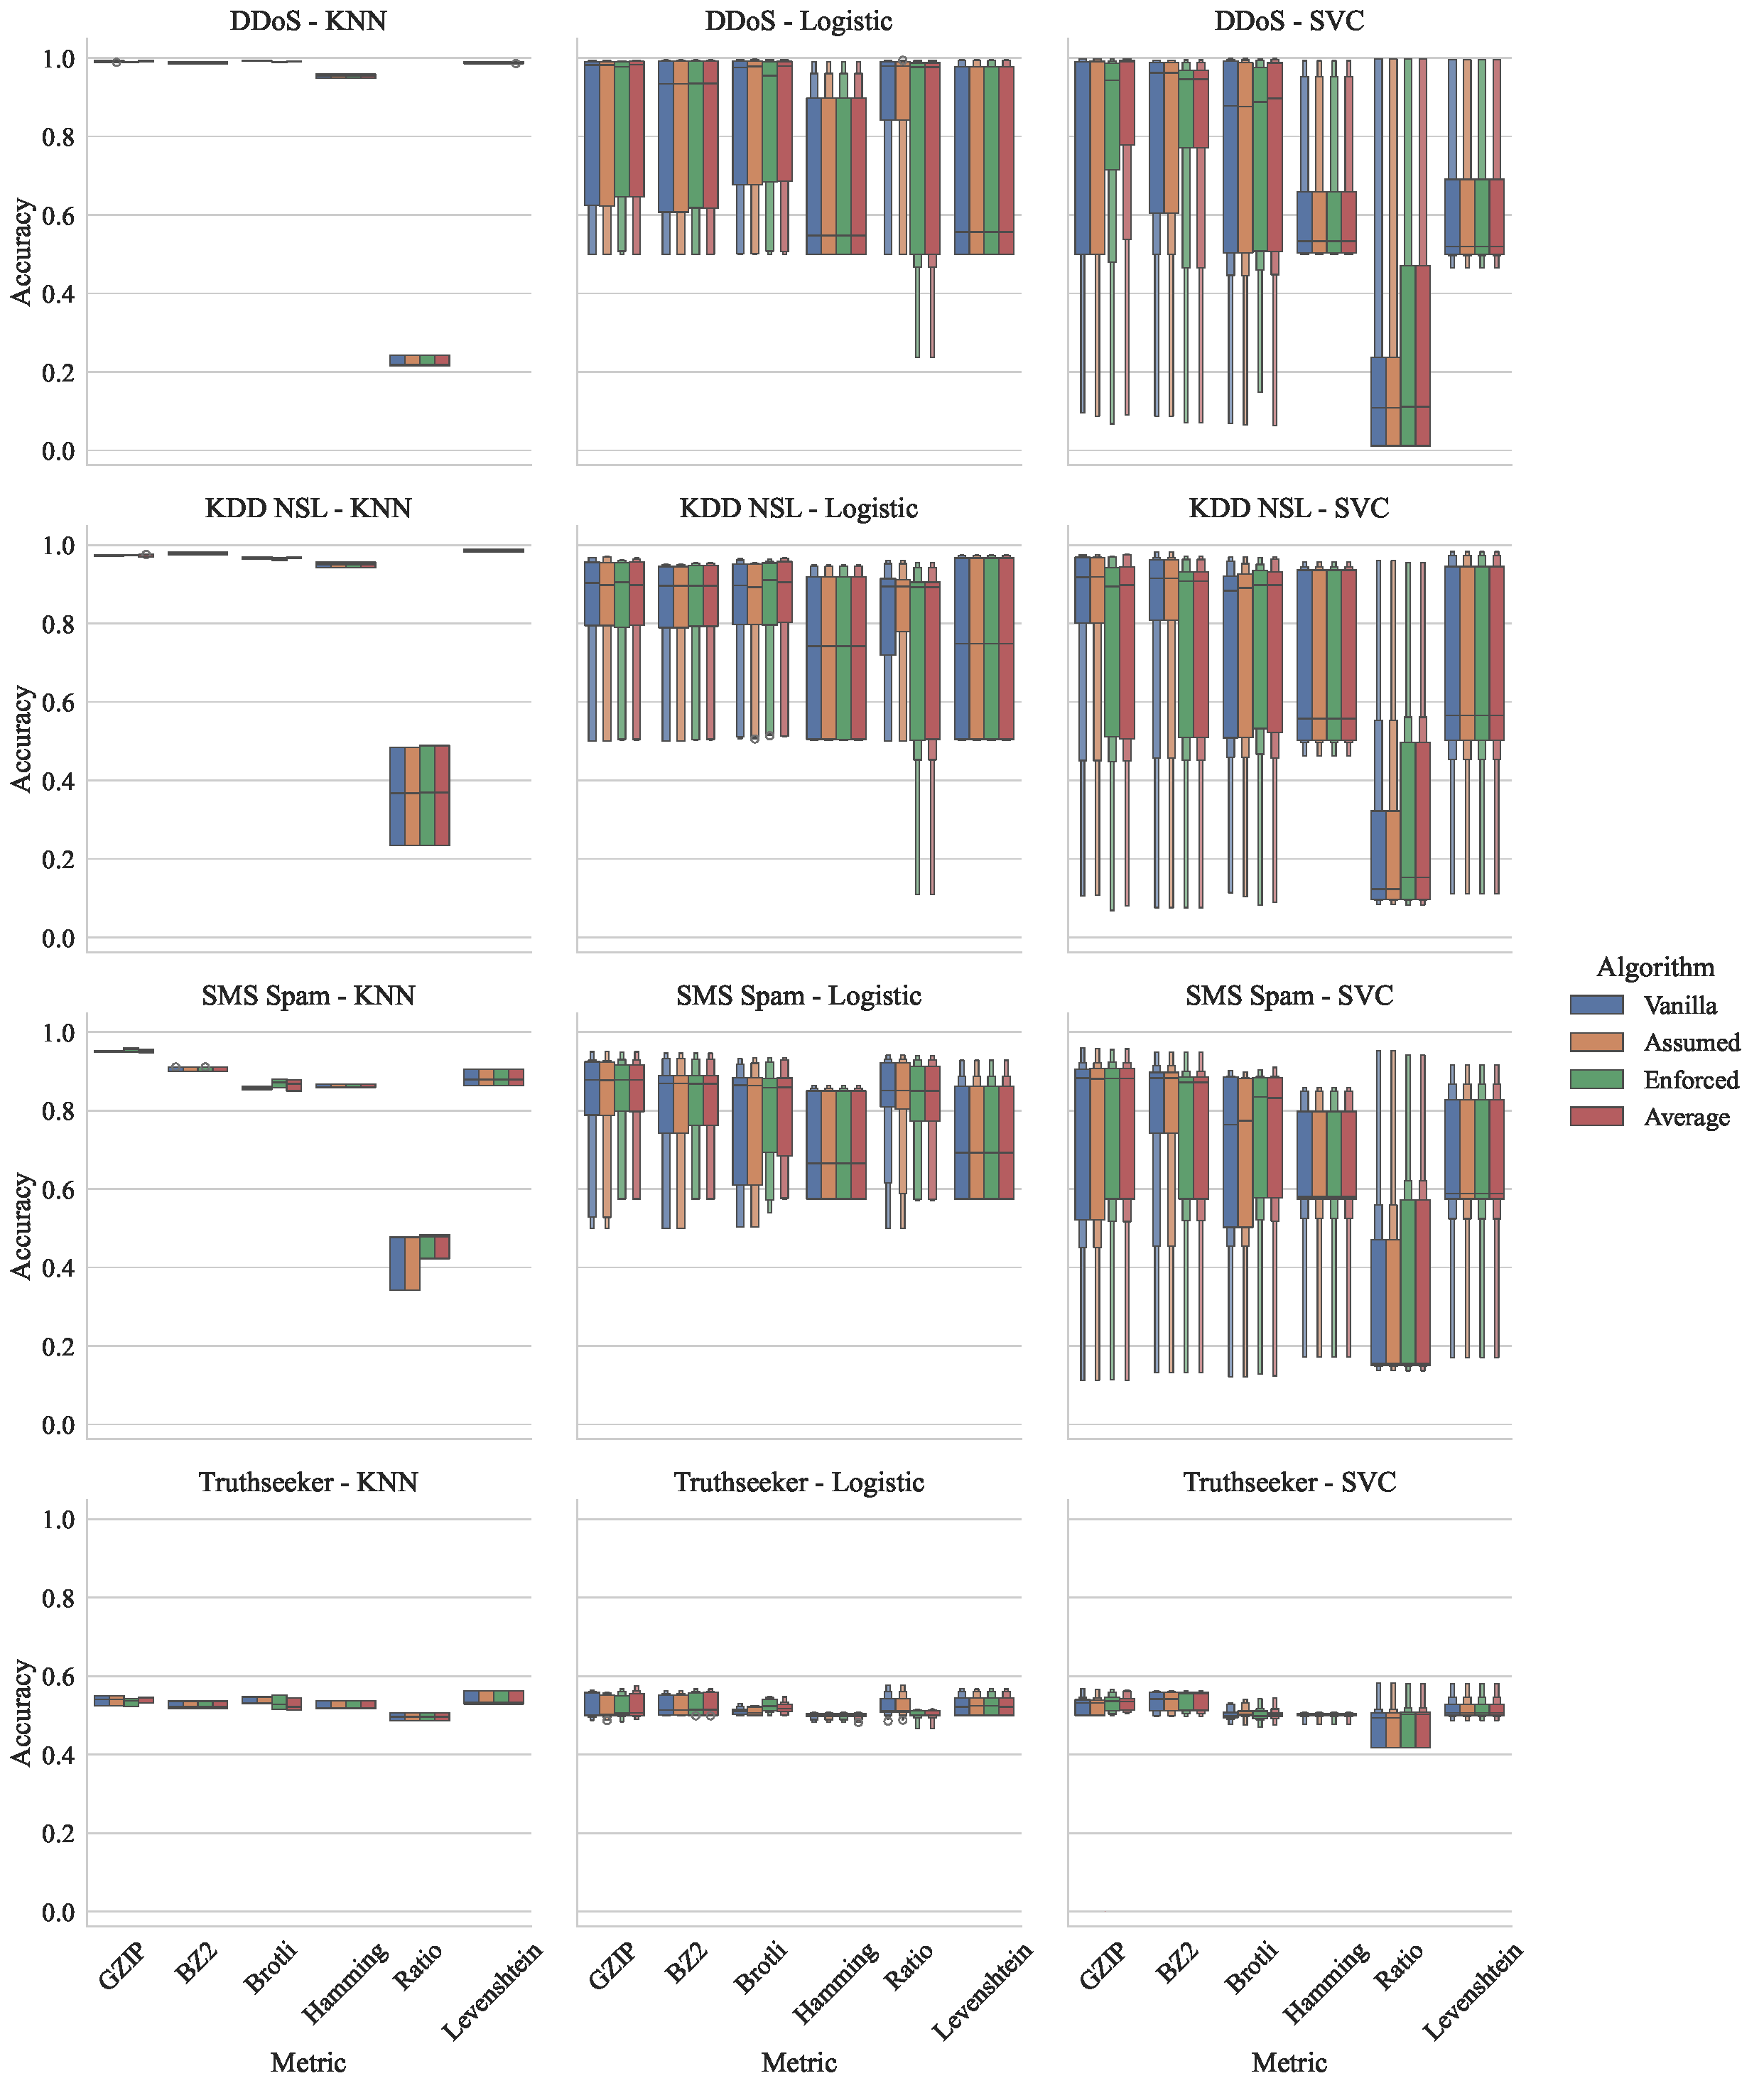
\includegraphics[width=\textwidth]{images/accuracy_vs_algorithm.pdf}
    \caption{The accuracy across each dataset (rows), model (columns) and distance matrix computation algorithm (color) for several different string metrics (x-axis).}
    \label{fig:metric_acc}
\end{figure*}

Figure~\ref{fig:metric_acc} shows the performance of the various classifiers (knn, logistic, SVC) across each of the datasets using various string metrics to calculate NCD. 
NCD using various compressors outperforms the string metrics across all datasets and classifiers. 
It is clear that run-times are largely comparable between NCD and various string metrics for both training (Figure~\ref{fig:train_time}) and inference (Figure~\ref{fig:pred_time}). 
Please note that the training step is only necessary for certain configurations of the KNN algorithm and that the vanilla version proposed by Jiang et. al.~\cite{jiang2022less} can skip this step entirely. 
Overall, NCD (GZIP, BZ2, Brotli) offers superior performance over the tested string metrics (Hamming, Ratio, Levenshtein) since NCD is more consistently accurate. Across all datasets, the median and peak accuracy of the compressor-based metrics exceeds all the string metrics.

\subsection{Effect of Kernelisation}

\begin{figure*}[htb]
    \centering
    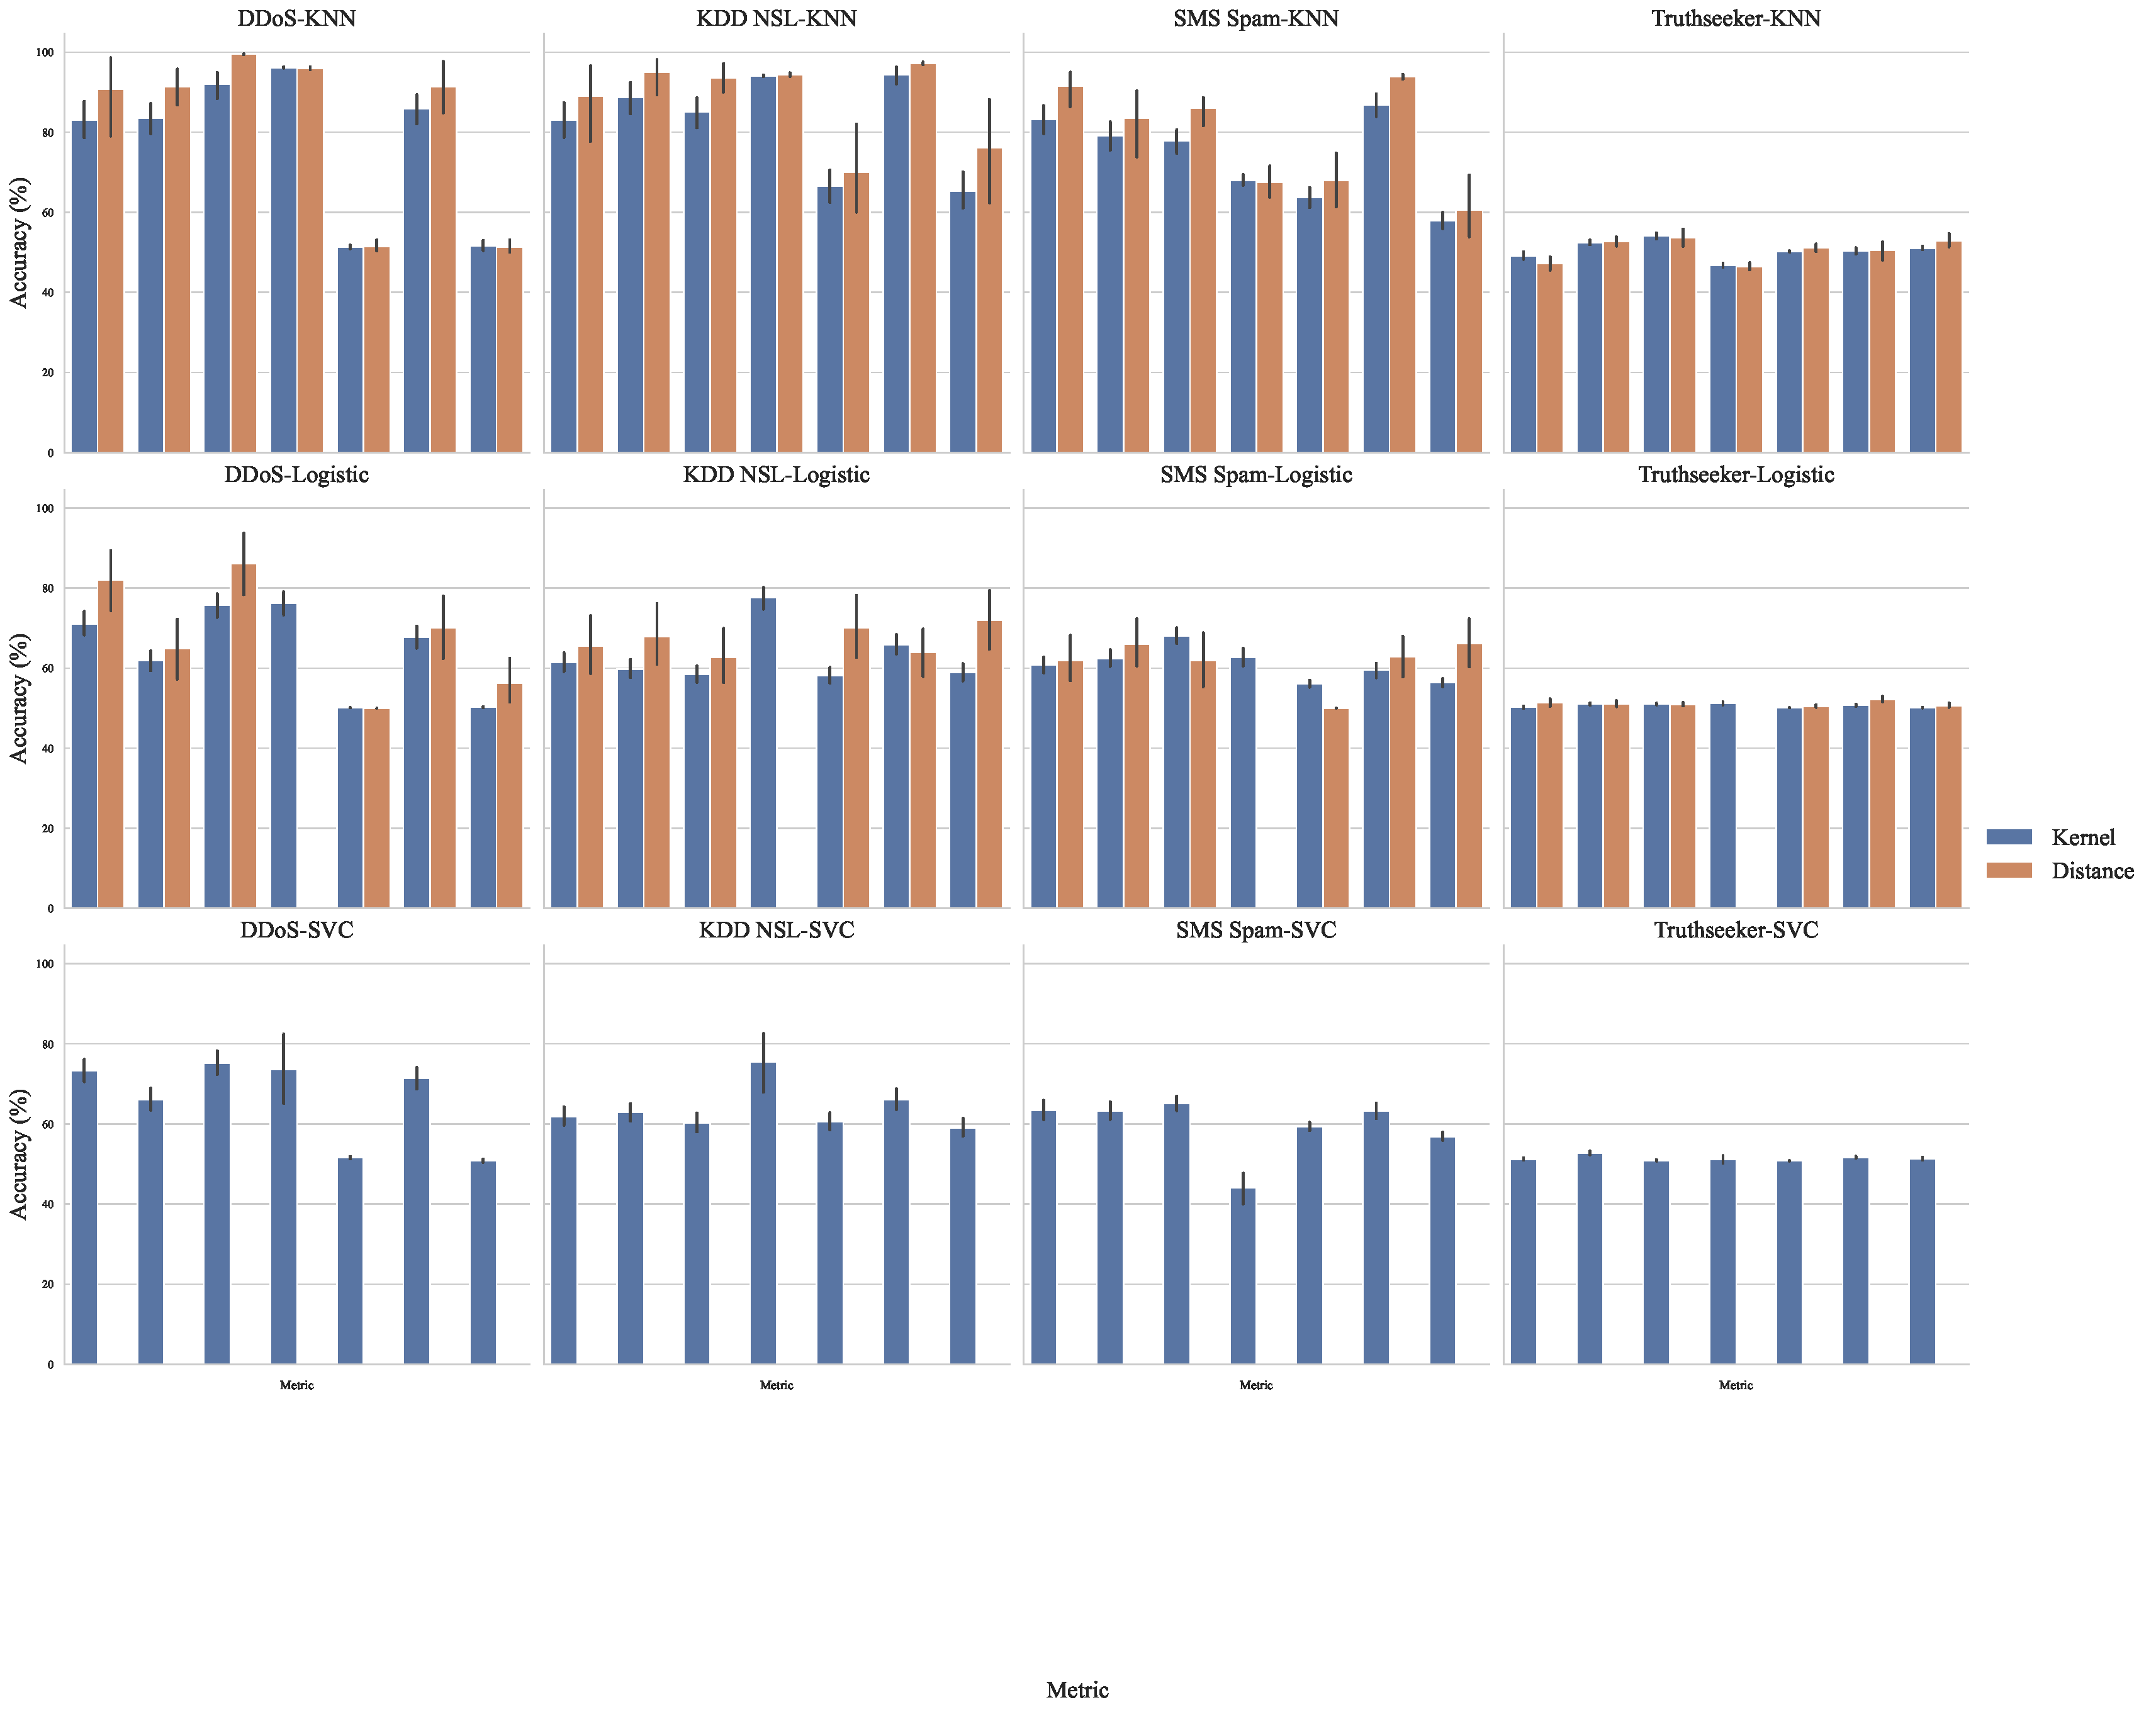
\includegraphics[width=\textwidth]{images/accuracy_vs_kernel.pdf}
    \caption{The accuracy across each dataset (rows), model (columns) and distance matrix computation algorithm (color) for several different kernelisation functions (x-axis), calculated by averaging the scores of each fold in five-fold cross validation for each set of tested parameters (enumerated in Section~\ref{models}).}
    \label{fig:kernel_acc}
\end{figure*}

Figure~\ref{fig:kernel_acc} shows the effect of kernelisation when compared to the un-kernelised distance matrix (on the far right side, denoted with a $D$) across all tested configurations of models across all the datasets. 
For KNN, the performance is identical for all datasets and models, which is not unexpected as the chosen kernel functions preserve the order of the neighbours, except when an (erroneous) negative distance occurs. 
As this situation is incredibly rare (see Figures~\ref{fig:mod_acc}~and~\ref{fig:kernel_acc}), it is not unexpected that the resulting accuracy remains the same. 
This trend is consistent across all of the datasets and distance matrix algorithms.
The kernelised logistic regressor fails to outperform the raw distance matrix, on average. 
However, after tuning, kernelised logistic regression can also approach perfect accuracy, but this comes at the cost of more tuneable parameters and a longer training time. 
This trend is also consistent across all of the datasets and distance matrix algorithms.
Unsurprisingly, the kernelised version of the distance matrix tends to outperform the un-kernelised distance matrix when used to build an SVC since that model is intended to work on similarity metrics (kernels) rather than dissimilarity metrics (distances). 
Like with logistic regression, this comes at the cost of one or more tuneable parameters and the resultant increase in training time. 
Nevertheless, this model might be more appropriate for situations in which the decision boundary is non-linear. 
Like with KNN and logistic regression, this trend is consistent across all datasets and distance matrix algorithms.


\subsection{Effect of Modified NCD Algorithm}

\begin{figure*}[htb]
    \centering
    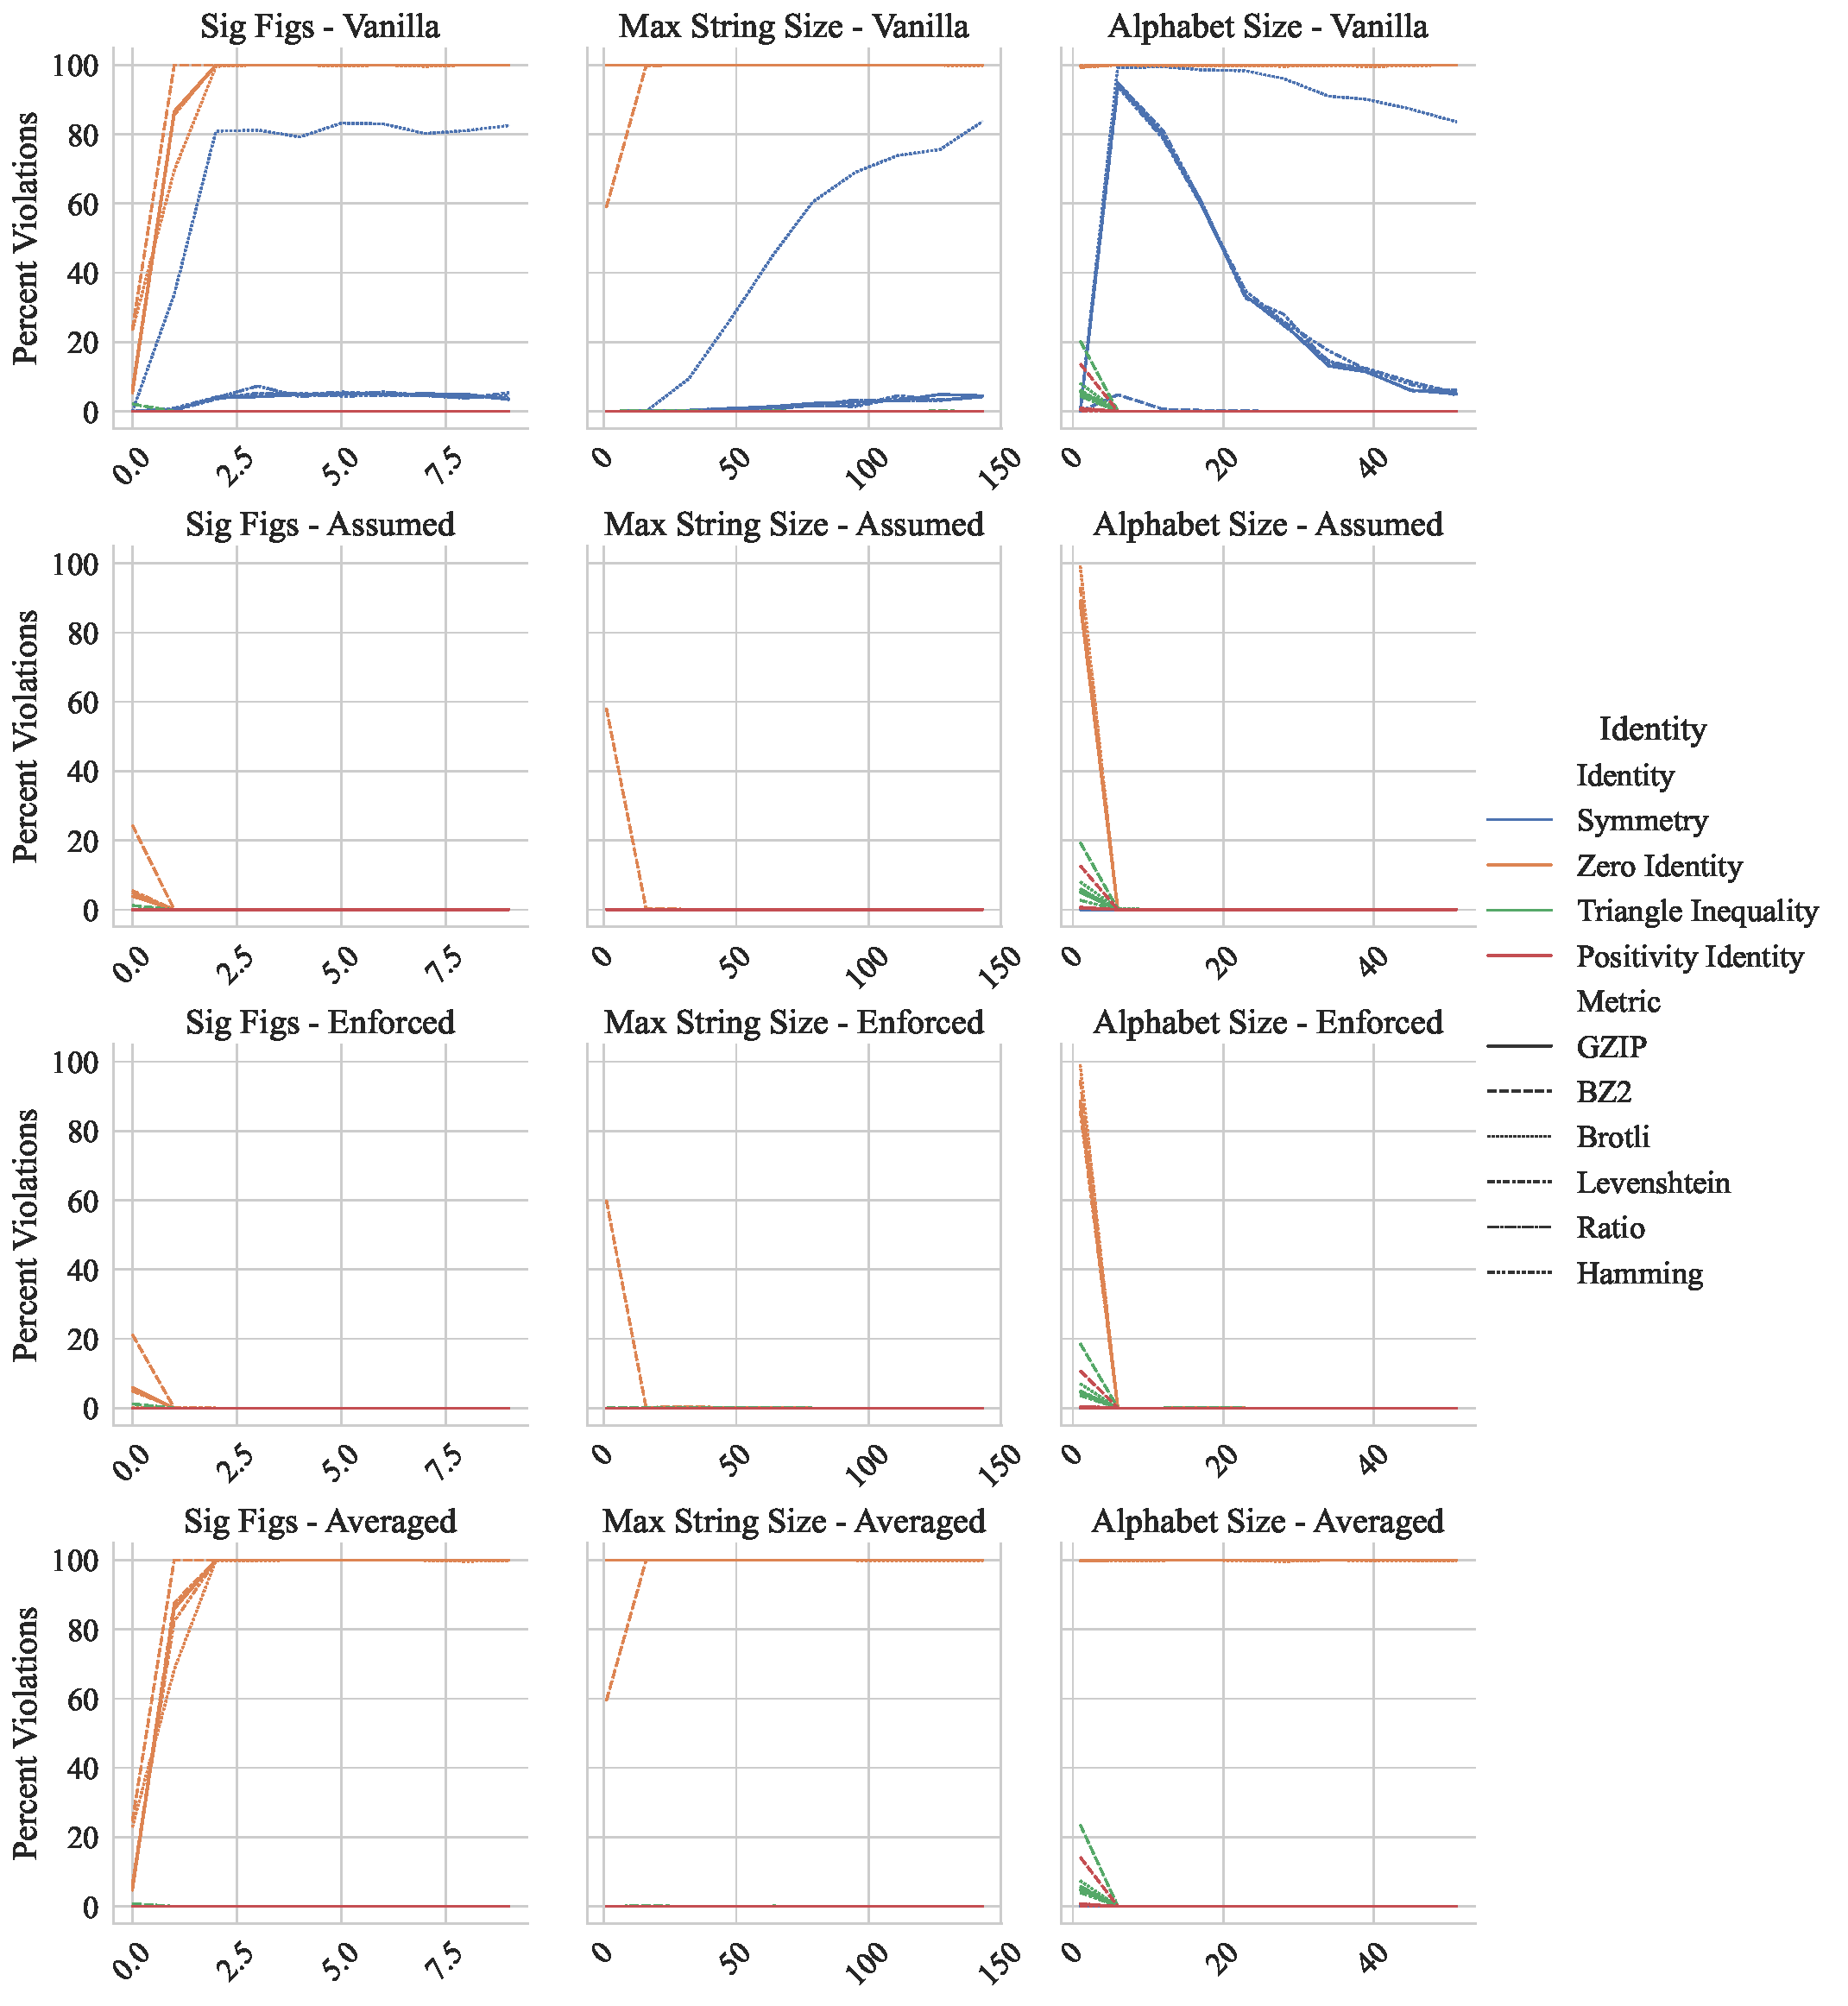
\includegraphics[width=\textwidth]{images/synthetic_check.pdf}
    \caption{
    Percentage of examples found that violate the assumptions outlined in Section~\ref{metric_spaces} using the vanilla (Algorithm~\ref{alg:vanilla}, top row), assumed symmetry (Algorithm~\ref{alg:symmetric}, second row), enforced (Algorithm~\ref{alg:modified}), and averaged (Equation~\ref{eq:average}) algorithms on 100 thousand random strings generated from the standard English alphabet (upper and lowercase). 
    \textit{Sig Figs} refers to the number of significant figures. \textit{Max String Size} and \textit{Max Alphabet Size} refer to the number of characters and the number of unique characters respectively. 
    Unless otherwise specified by the x-axis in an individual plot, \textit{Max String Size}, \textit{Max Alphabet Size}, and \textit{Sig Figs} were all 144 characters (the character limit of a ``tweet''), 52 letters (upper and lower case English letters), and 10 significant figures. Each colour corresponds to a different identity as defined in Section~\ref{metric_spaces} and each line marker corresponds to a different compression algorithm as outlined in Table~\ref{tab:compression_algorithms} and Section~\ref{string_metrics}.
    }
    \label{fig:synthetic_check}
\end{figure*}

\begin{figure*}[htb]
    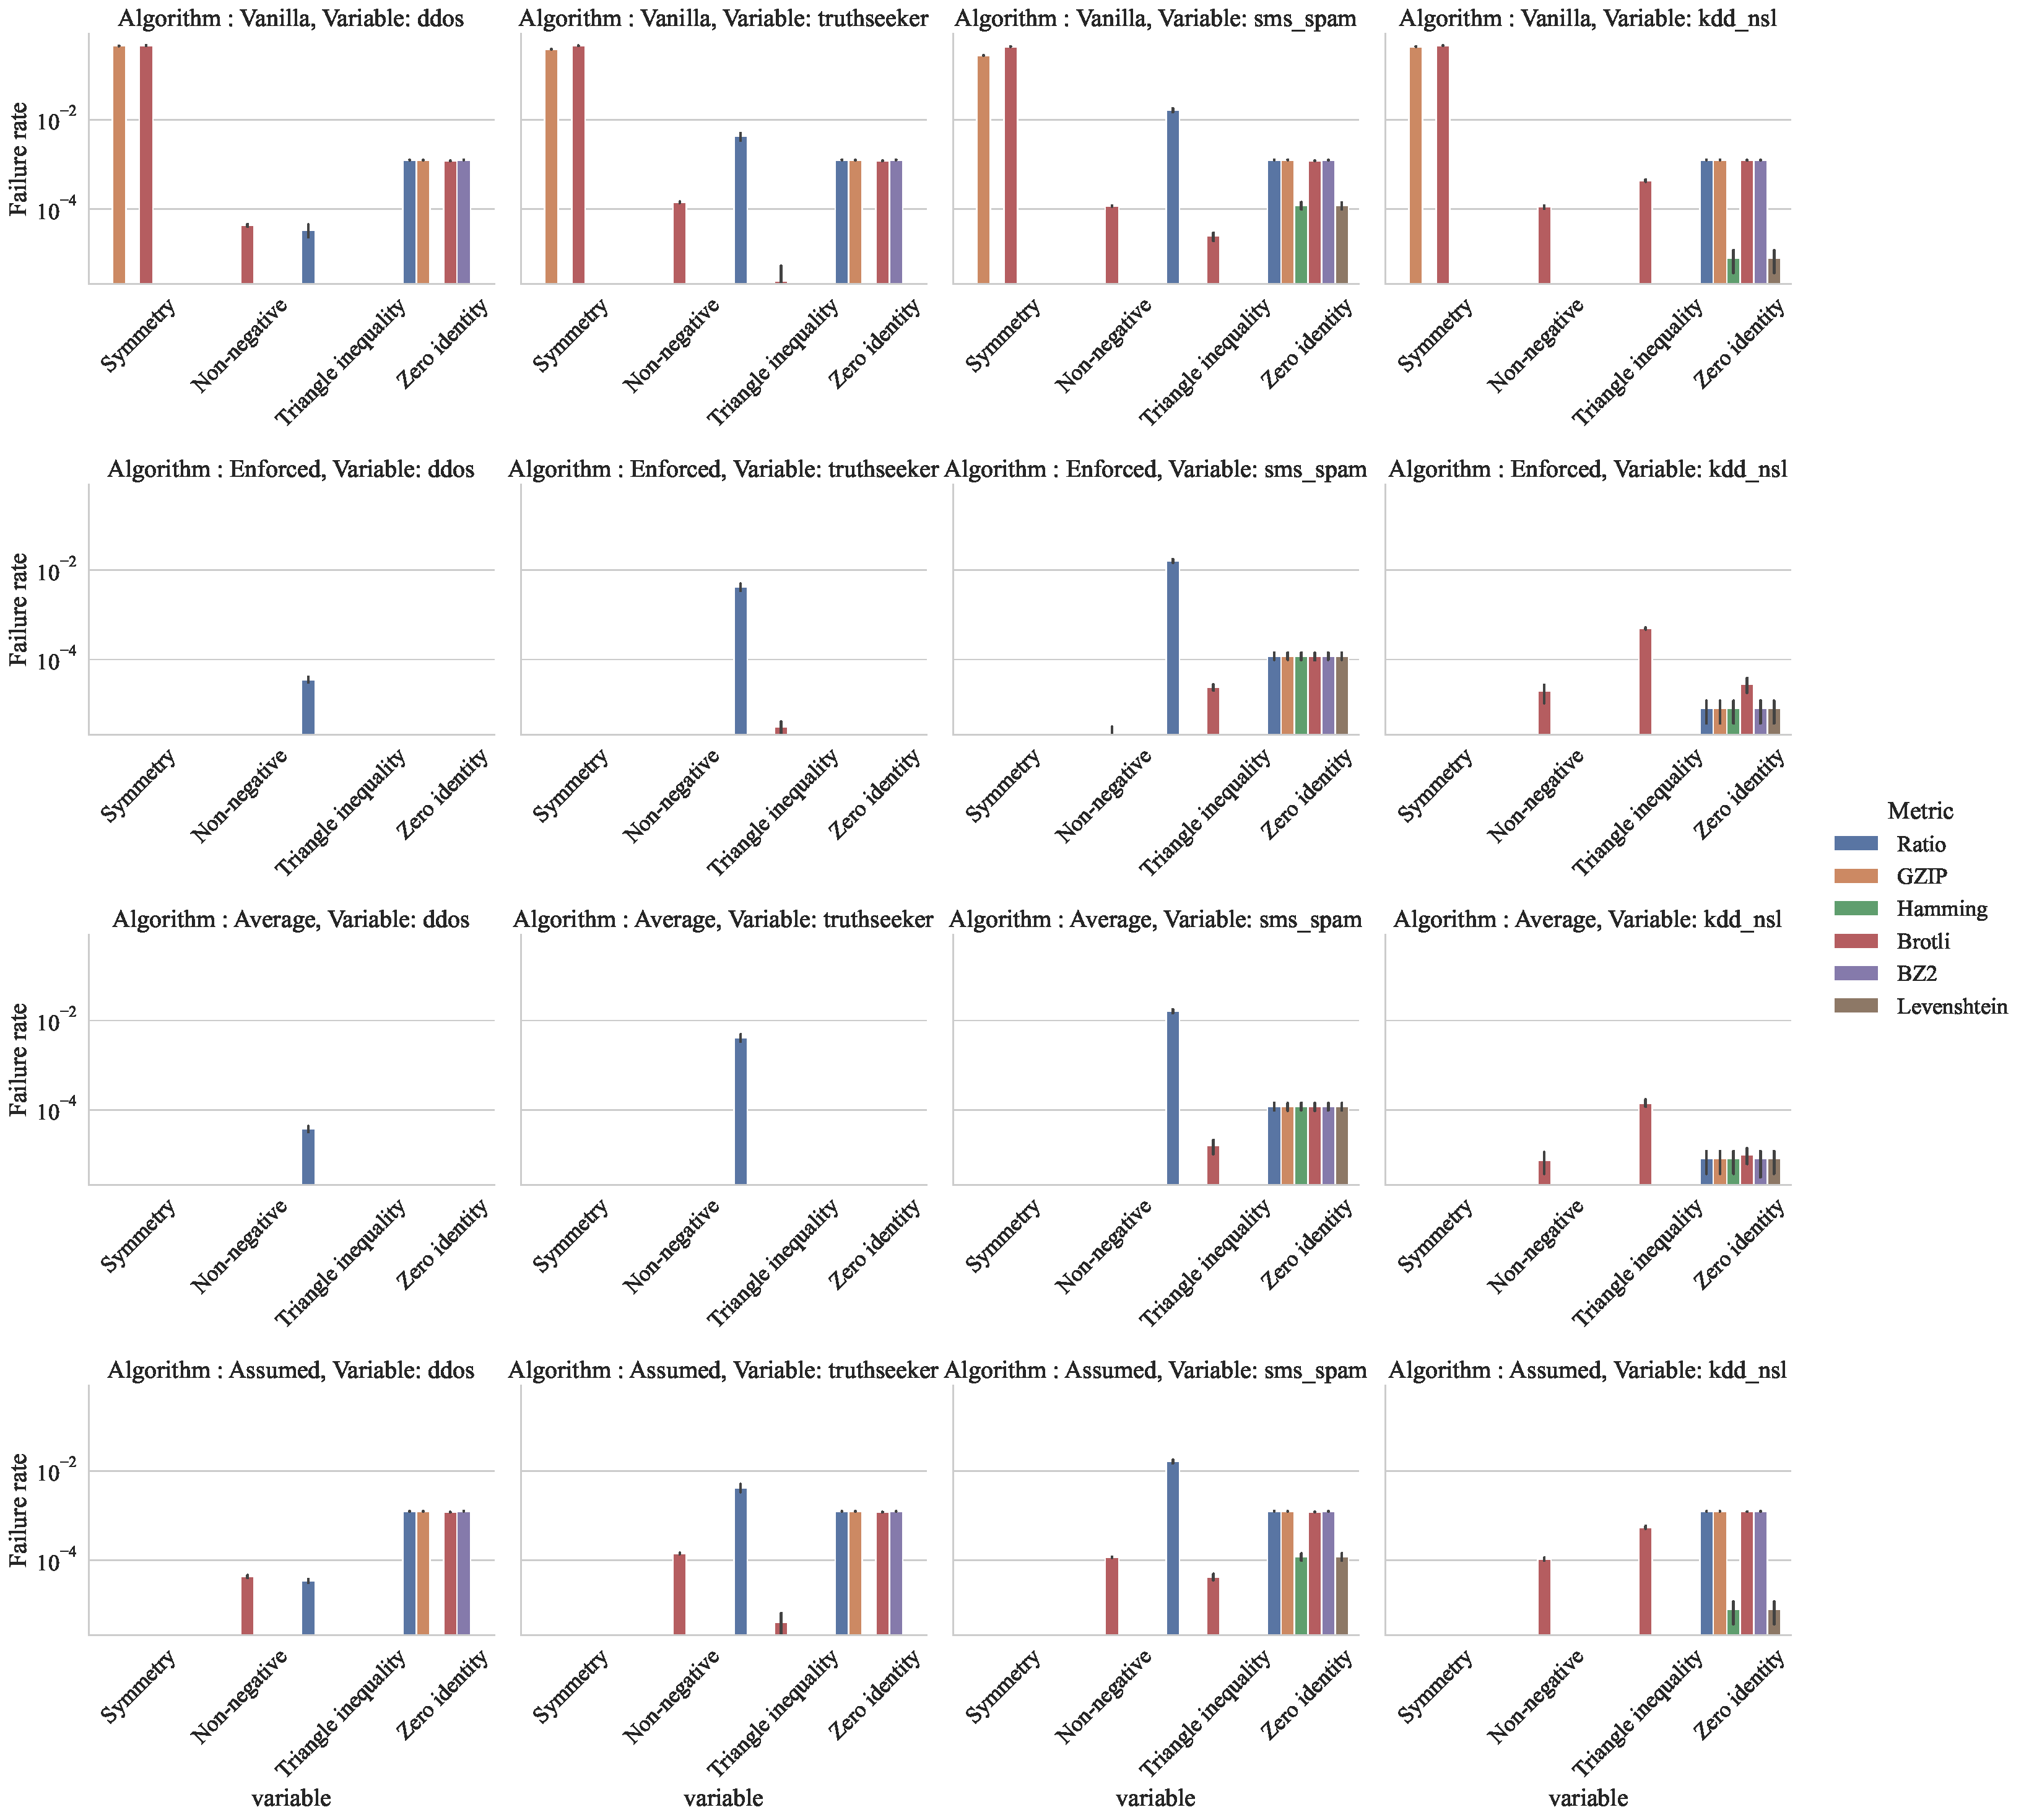
\includegraphics[width=\textwidth]{images/read_world_check.pdf}
    \caption{Percentage of examples found that violate the assumptions outlined in Section~\ref{metric_spaces} using the vanilla (Algorithm~\ref{alg:vanilla}, top row), assumed symmetry (Algorithm~\ref{alg:symmetric}, second row), enforced (Algorithm~\ref{alg:modified}), and averaged (Equation~\ref{eq:average}) algorithms on the training matrices for each of the outlined datasets. Each column is dedicated to a dataset and each model is given a column. The x-axis displays which of the identities is violated and the colour indicates which distance matrix algorithm was used. Since evaluating all possible distance 3-tuples would be computationally infeasible for even hundreds of samples, three disjoint distances were sampled  100 thousand times.}
    \label{fig:real_world_check}
\end{figure*}

Figures~\ref{fig:metric_acc}~and~\ref{fig:kernel_acc} depict the accuracy (top), Figure~\ref{fig:train_time} depicts the   training time per sample, and Figure~\ref{fig:pred_time}  depicts the inference time per sample (bottom) for each algorithm (denoted by color and outlined in ~\ref{extensions}). 
The accuracy of the modified algorithm is fairly consistent with the unmodified version. 
In practice, the model builder would choose the most accurate model, which is consistent across the algorithms and classifiers for each dataset. 
However, the modified version of the algorithm is clearly much faster per sample when constructing the distance matrix ($t_t$) by reducing the number of distance computations by a factor of 2. 
This comes at the marginal cost of a few hundred milliseconds for each prediction, however, but this could easily be mitigated by skipping the algorithmic modifications during the prediction step and handle the problem of negative distances at run-time, depending on the particular application. 
Overall, it is clear that this modified version of NCD offers significant run-time improvements while costing nothing in terms of accuracy. 
Additionally, by running the vanilla version during prediction and using the modified version if and only if the distance matrix is calculated, these downsides can be avoided entirely. 
However, that may produce distance matrices that are incompatible with other tooling or models (see: Figure~\ref{fig:synthetic_check}, middle row), most of these are mitigated with the proposed modifications (see: Figure~\ref{fig:synthetic_check}, bottom row). 
However, two classes of counterexamples remain. 
The first occurs with very short strings
$NCD("ABB", BBBB) =0$ because the marginal length associated with the repeated ``BB'' token happens to be the exact length as the marginal length associated with the token ``A''. 
This second occurs for the triangle inequality. 
Letting $x =AACAABC, y = AA,
z=AAA$, we find that $NCD(x,y) \approx .26$ while $NCD(x,z) + NCD(z,y) \approx .23$, but it's not clear that this is a problem in the theory. Including the string ``AAA'' provides additional context that ``AA'' may have a distinct meaning apart from ``A'' repeated twice which is why the distance of the sum \textit{is} less than the distance between $x$ and $z$. Additionally, it doesn't seem to be a problem in practice. 
As the max string size or the maximum alphabet size is increased, these problems quickly disappear(see: Figures~\ref{fig:synthetic_check}~and~\ref{fig:real_world_check}.


\subsection{Run-time Considerations}

Figure~\ref{fig:train_time} depicts the time needed to calculate the distance matrix per sample in the training set for each dataset (column), algorithm (colour) and metric (x-axis). 
It is clear that the run-times of the metrics are fairly consistent across the datasets and that the proposed run-time improvements (denoted ``Assumed'' and ``Enforced'') do decrease the training time with no resulting loss in accuracy (see: Figure~\ref{fig:metric_acc}). 
While the symmetric extension of NCD (denoted ``Averages'') does take significantly more time thant the other distance matrix algorithms, that marginal increase is mere milliseconds in practice and is guaranteed to be symmetric without assuming or enforcing symmetry. 
However, Hamming distance takes significantly more time than other metrics on the DDoS dataset and GZIP takes significantly more time than other metrics on the KDD NSL dataset. 
This effect can be mitigated by considering the run-time costs during the model training stage since these metrics take longer but do not result in significantly better accuracies (see: Figure~\ref{fig:metric_acc}) for those datasets. 
Overall, training times are low enough that this could feasibly be deployed on a user's device without specialised hardware (as is true in the case of neural networks). 
If we pessimistically assume a training time of 50 milliseconds per sample, then training could occur as the user (or router or antivirus software or social media algorithm) encounters the sample in real-time with a latency that would be unnoticeable to most humans (roughly a few hundred milliseconds, depending on age and other factors)~\cite{reaction_time}. 
Figure~\ref{fig:pred_time} depicts the time needed to predict a new classification on a single sample for each dataset (row), classifier (column), algorithm (colour) and metric (x-axis). 
The prediction time per sample (after calculating the distance between a new sample and those in the training set) is trivial across all distance matrix algorithms, datasets, models, and metrics, though the branching logic introduced by the ``Assumed'' and ``Enforced'' algorithms does increase the model latency by a fraction of a millisecond.
Overall, it is clear that the run-time improvements are effective and that NCD is can be plausibly used in real-time, client-side settings. 
In applications where latency is more important than privacy, then the training distance matrix can be pre-computed (rather than generated at run-time as in unweighted KNN), reducing the run-time and computational costs for the user. 



\begin{figure*}[htb]
    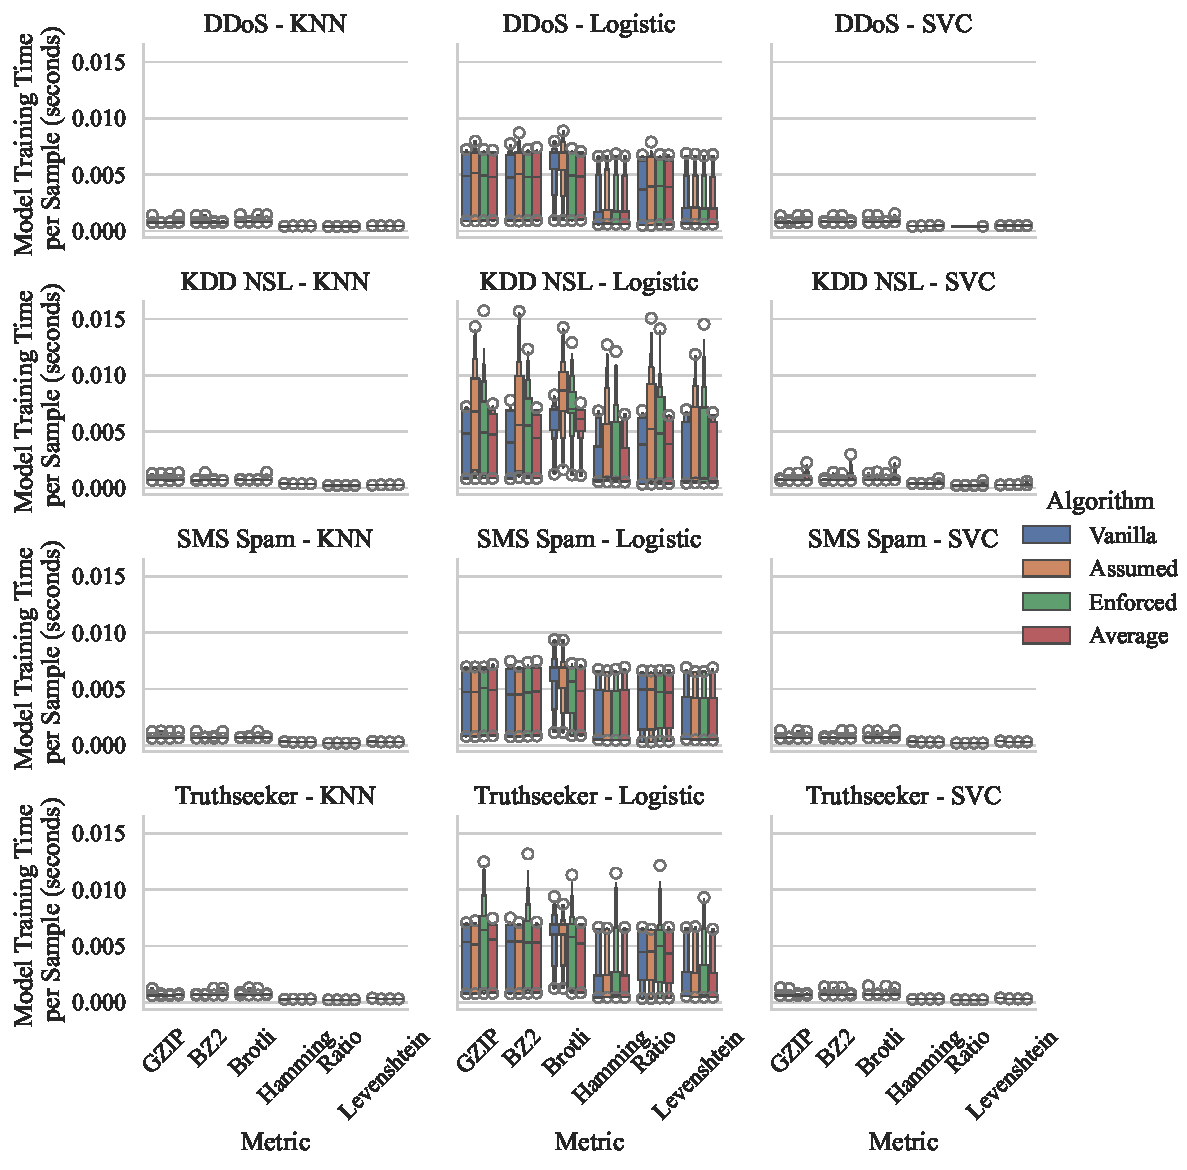
\includegraphics[width=\textwidth]{images/train_time_vs_algorithm.pdf}
    \caption{The distance matrix calculation time per sample for each metric (x-axis), dataset (columns) and algorithm (colour). Because the distance matrix was only calculated once per dataset, there is no differentiation between the models. Likewise, this time was much, much larger than the time needed to fit each model, making the choice of algorithm and metric the primary run-time concerns.}
    \label{fig:train_time}
\end{figure*}

\begin{figure*}[htb]
    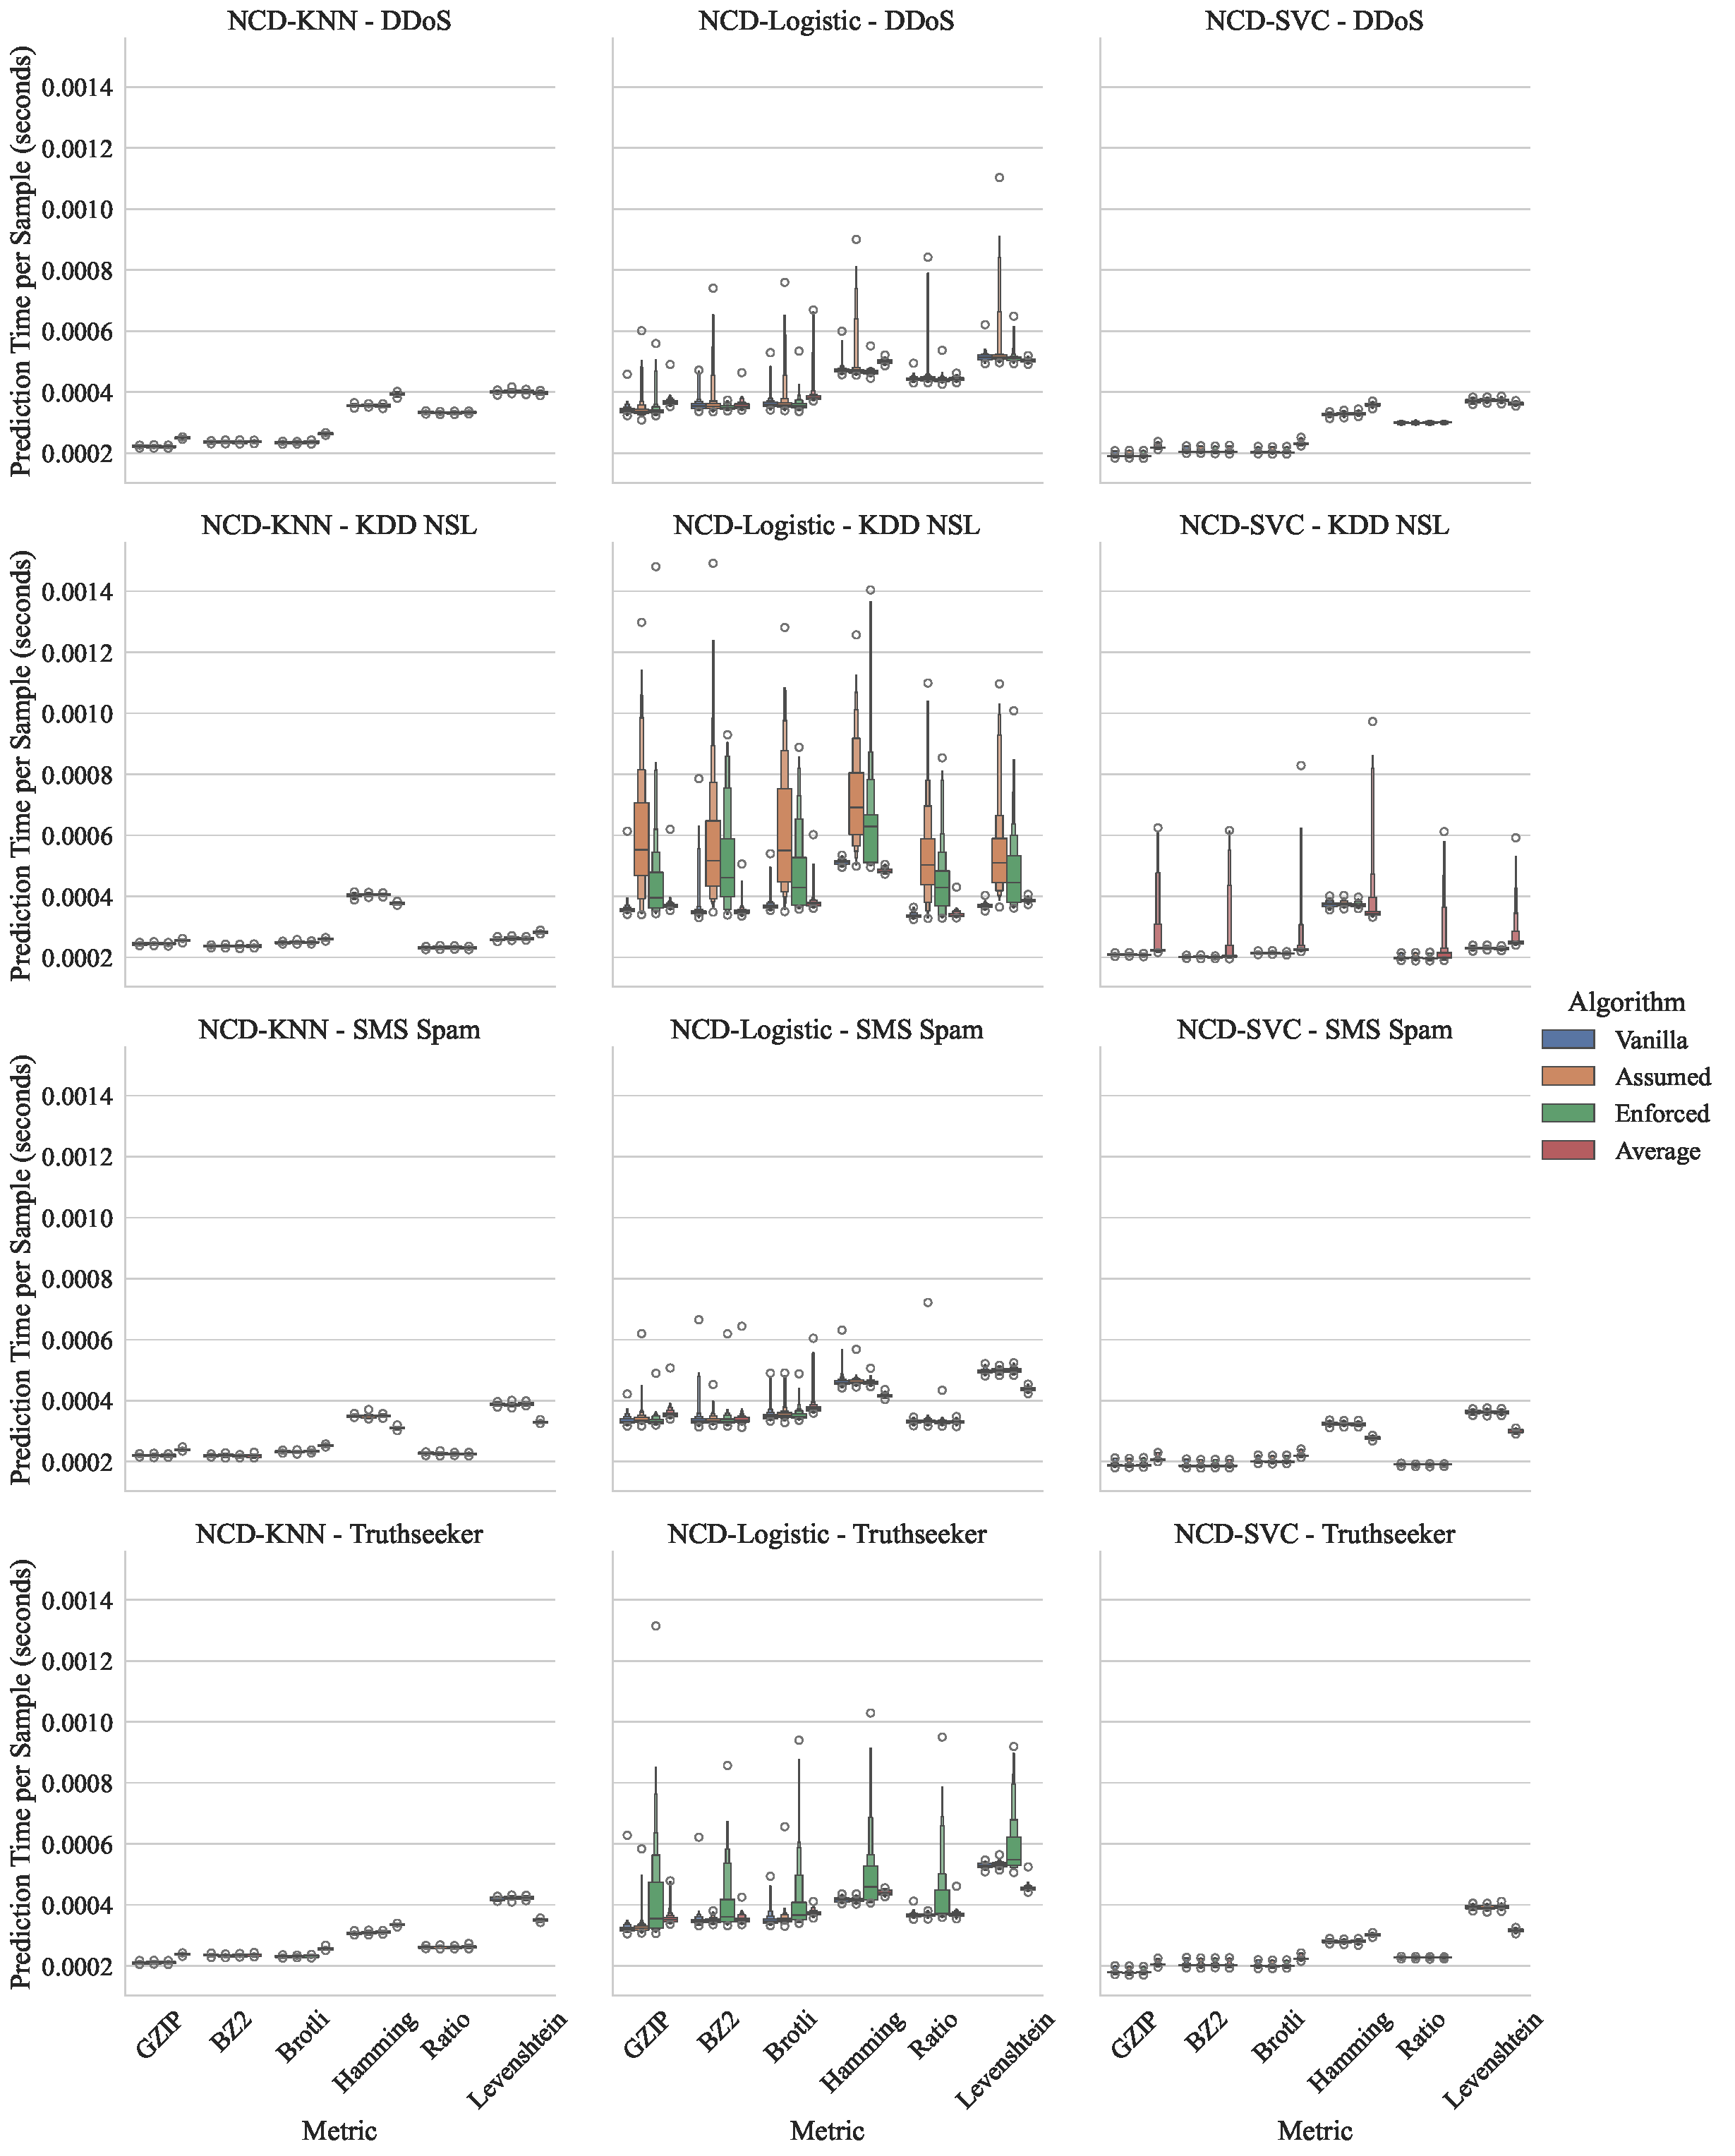
\includegraphics[width=\textwidth]{images/pred_time_vs_algorithm.pdf}
    \caption{The predictions time per sample for each metric (x-axis), dataset (rows), models (columns), and algorithm (colour).}
    \label{fig:pred_time}
\end{figure*}



\section{Considerations}
\label{considerations}
While the proposed algorithm (see \ref{alg:modified}) does improve upon certain edge cases outlined in Section~\ref{pseudometric}, the examined condensing methods (see: Section~\ref{extensions} do not have any significant effect on model performance (see: Figures~\ref{fig:metric_acc}~and~\ref{fig:kernel_acc}). 
However, the vanilla NCD-KNN proposed by Jiang et. al.~\cite{jiang2022less} remains an effective choice if the training step is deemed too expensive for the chosen applications and the only reason to deploy the extensions would be to reduce the training time--- an unnecessary step for unweighted KNN. 
Here, the authors would like to note the borderline performance of all metrics on the Truthseeker dataset---both NCD and more traditional distance measures. However, this is on par with the performance from the original authors~\cite{truthseeker}. To the best knowledge of the authors, most content on the platform formerly known as Twitter is simply indistinguishable from bot-generated spam---using any known distance metric.


\section{Conclusion}
\label{conclusion}

It is clear from Figures~\ref{fig:metric_acc}-\ref{fig:train_time} that the extensions proposed in this work are superior to the method proposed by Jiang et. al. when applied used a distance measure for kernelised classifiers. 
By pre-emptively handling cases that would result in negative values for distance (thus violating the Non-negativity identity) and sorting the inputs, this modified NCD is guaranteed to behave more like a true metric. 
This allows the model builder to use standard tooling (e.g.~\texttt{scikit-learn},~\texttt{imblearn}) to build classifiers that perform well on an exceedingly small number of samples. The end result is a real-time, client-side classification algorithm that doesn't rely on federation, centralization, or the large scale processing of millions of data points across a global user-base. 
This categorically circumvents poisoning attacks~\cite{biggio_poisoning_2013} since each labelled database is unique to each user. 
Furthermore, this reduces the attack surface of attacks like model inference attacks, database exfiltration attacks, and evasion attacks since a malicious user would need to target the personalised classifier of each user~\cite{biggio_evasion_2013,deepfool,chakraborty_adversarial_2018}. 
While it is known that some attacks are quite transferable~\cite{wang2021enhancing}, this reduces the common attack surface to \textit{only} the samples that are universal across the user base and a new model can be generated trivially by refreshing the page or appending the offending sample to the labelled (training) dataset. 




\bibliographystyle{ieeetr}
\newpage
\bibliography{bibliography}


\end{document}
